\chapter{Hardware}
\label{hardware_chapter}

This chapter will present the hardware modules and will explain the tools used to design them, as well as the existing work in which our design is based. The modules are composed of a mechanical part, a electronic control board, and other elements such as the servo or the battery, that will be explained on their corresponding sections on this chapter.\\

%%%%%%%%%%%%%%%%%%%%%% MODULE %%%%%%%%%%%%%%%%%%%%%%%%%%%%%%%%%%%%%%%%%%%%
\section{Module}
\label{hardware_module}
In this section we will talk about the design of the mechanical part of the module, the two-piece plastic structure that holds the servo and transmits its movement to the other modules, allowing the modular robot to move. We will start discussing the modelling paradigm used to design the model, then we will introduce the previous existing modules from which we took inspiration to design our module, and finally we will present our design, with the corresponding assembling instructions.\\

%%%%%5555%%%%%%%% software used %%%%%%%%%%%%%%%%%%%%%%%%%%%%%%%%%%%
\subsection{Software used}
\label{hardware_software_used}

The approach tipically followed for the design and modelling of 3D object is usually a interactive one. Using a CAD software such as SolidWorks the engineer designs the object by applying a series of transformations to a basic shape until the final object is obtained. Other approach, not so frequently employed, is generative design. With this approach, the object is generated by a set of rules or an algorithm, like a computer program. This way, the design can be specified as a function of a set of variables or parameters that can be later modified, modifying the whole design and varying its dimensions, or generating different parts or variations of the same parts. \\

Using this generative design paradigm, we have designed a module that is parametric, and whose 3D model adapts automatically to the servo and control board, allowing the design to be more accessible, as it does not depend on a single servo model and reusable, as it can adapt to the user needs.\\

\subsubsection{OpenSCAD}
\label{hardware_software_openscad}
OpenSCAD is an open source software for creating solid 3D CAD objects \cite{openscad:website}. Unlike most 3D object editors, it is not interactive, but based on script files that describe the geometry from operations with basic primitives.\\

It provides two main modelling techniques: Constructive Solid Geometry (CSG), where boolean operators are applied to primitive 3D objects to create complex 3D objects; and extrusion of 2D outlines, where a 2D shape is extruded to create a 3D object. This techniques can be mixed, using 3D objects generated by extrusion of 2D outlines as operands of boolean operators to generate even more complex geometries.\\

CSG modelling has several advantages over the use of polygonal meshes. With CSG modelling the user can model very complex geometries with just a reduced set of simple primitive objects, simplifying the modelling process. If GSG is procedural or parametric, a complicated design can be changed easily by changing the parameters, allowing designs to be adapted to the new requirements automatically. When the primitive objects used in CSG modelling are ``solid'' or water-tight it is ensured that the resulting object is also water-tight, which is very important for manufacturing the object. As opposed, when creating geometries using  polygonal meshes, consistency checks must be performed to ensure that the mesh represents a valid solid object. Finally, a point can be easily classified as being inside or outside the resulting shape by testing it against all the underlying primitives, and evaluating the boolean expression that generated the shape with the classification values, which is very useful in applications such as collision detection.\\

The 3D primitives available for CSG in OpenSCAD are three: cube, cylinder and sphere. Cones can be generated from cylinders by specifying a top/bottom radius of 0 units when creating it. These primitive shapes can be translated, rotated or scaled any number of times, and then boolean operators can be applied to form complex shapes. OpenSCAD has boolean operators for performing unions, differences and intersections of objects. Figure \ref{fig:hardware_openscad_example} shows an example of a complex object assembled from simple combinations of primitive objects and boolean operations.\\

\begin{figure}[h]
		\centering
        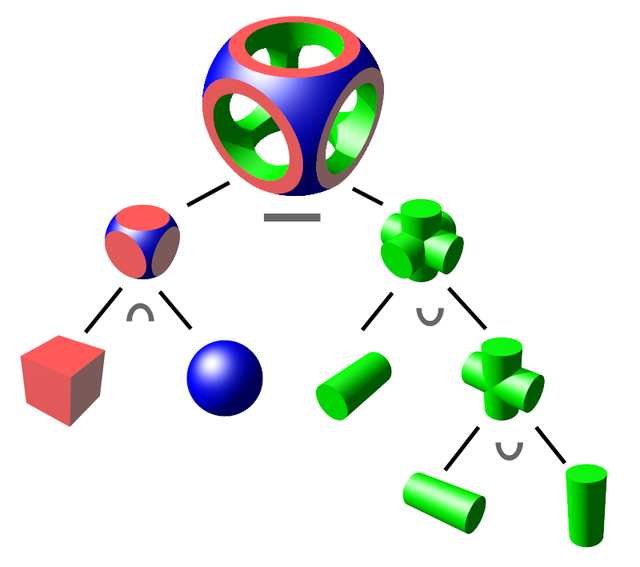
\includegraphics[width=0.4\textwidth]{images/Hardware_openscad_example.png}
        \caption{Example of a complex shape made from simple primitive objects and boolean operators.}\label{fig:hardware_openscad_example}
\end{figure} 

OpenSCAD also counts with some 2D primitives for creating objects through 2D shape extrusion, such as squares, circles and polygons, defined point by point. It also can import CAD files in DXF format for extruding them, or export 2D shapes in DXF format to use them in other CAD programs. The 2D shapes can also be combined using boolean operators, and the extruded to form 3D objects, either with a linear extrusion or with a rotate extrusion, that creates solids of revolution.\\

\begin{figure}[h]
		\centering
        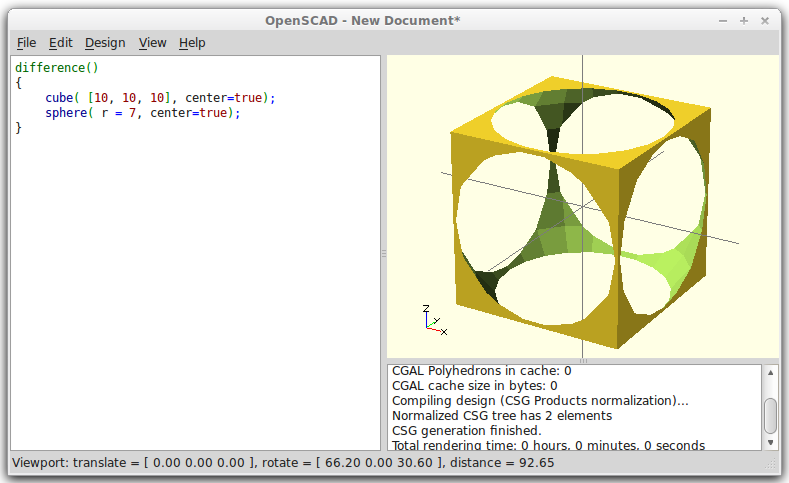
\includegraphics[width=0.7\textwidth]{images/Hardware_openscad_example2.png}
        \caption{OpenSCAD screenshot with a simple object being created.}
        \label{fig:hardware_openscad_example2}
\end{figure} 


%%%%%%%%%%%%%%%%%%%%%%%%%%%%%%%%% OOML %%%%%%%%%%%%%%%%%%%%%%%%%%%%%%%%%%%%%%%%%%%%%%%%%%%%%%%%%%%%%%%%%%%%
\subsubsection{Object-Oriented Mechanics Library (OOML)}
\label{hardware_software_ooml}

The Object-Oriented Mechanics Library \cite{ooml:website, Valero-Gomez2012} is an open source C++ library to model 3D objects using C++, in a similar way as the objects are described with OpenSCAD. It was developed by Juan Gonzalez-Gomez and Alberto Valero-Gomez as a way to extend the capabilities of OpenSCAD with the features available in more advanced programming languages such as objects, inheritance or operator overloading, as well as the existing libraries for those languages to, for example, perform mathematical operations.\\

OOML counts with the same primitive 3D objects of OpenSCAD (cube, cylinder and sphere), plus some additional components such as toroids, prisms, rounded tablets, rounded cubes, rounded cylinders or text strings. It also offers the same 2D primitives, and boolean operations, that can be performed with the classic C++ operators: ``$+$'' for union, ``$-$'' for difference and ``$*$'' for intersection.\\

Apart from the basic primitive objects, OOML has also a part library with 
more complex, basic objects with a mechanical meaning, that can be combined to form even more complex mechanisms, such as robots. These objects are parametric, so they can be reused across designs, and derivative objects can be made based on these ones by using C++ inheritance. This library contains wheels, battery holders, batteries, servos, sensors, etc.\\

\begin{figure}[h]
		\centering
        \begin{subfigure}[b]{0.49\textwidth}
                \centering
                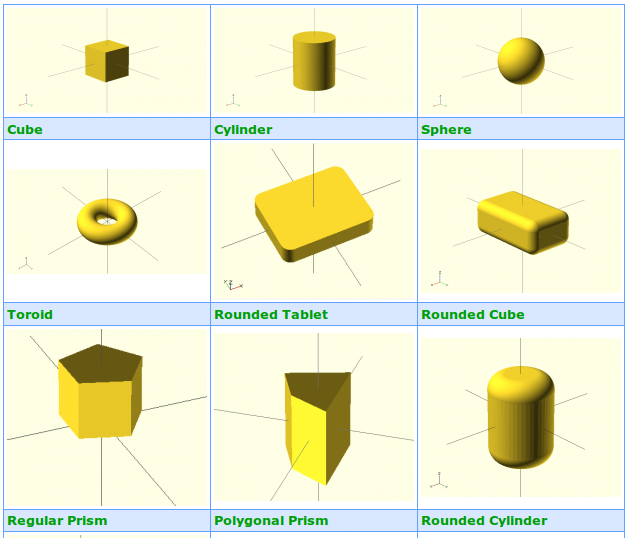
\includegraphics[width=\textwidth]{images/Hardware_ooml_primitives.png}
                \caption{Primitive objects}
                \label{fig:hardware_ooml_primitives}
        \end{subfigure}
        ~
        \begin{subfigure}[b]{0.45\textwidth}
                \centering
                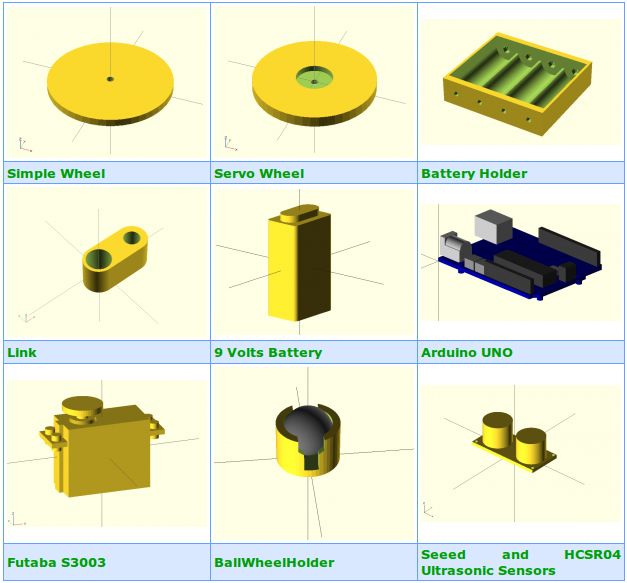
\includegraphics[width=\textwidth]{images/Hardware_ooml_parts.png}
                \caption{Parts}
                \label{fig:hardware_ooml_parts}
        \end{subfigure}
        \caption{OOML's primitive objects and parts}
        \label{fig:hardware_ooml_example}
\end{figure}

From the compoment object, OOML automatically generates OpenSCAD code that can be used to render and compile the object in the OpenSCAD development environment. For the code generation OOML has a class, called \emph{Writer}, that is in charge of converting the description of a 3D object into OpenSCAD code.\\

%%%%%%%%%%%%%%%%%%% Previous work %%%%%%%%%%%%%%%%%%%%%%%%%%%%%%%%%%%%%%%%%%%%
\subsection{Previous work}
\label{hardware_previouswork}

On the state of the art, we introduced several platforms for developing modular robotics. For developing our module we reviewed all of them, and we decided not to reinvent the wheel starting a new design from scratch, so we selected an existing open platform, the Y1 module and its derivatives.

\subsubsection{Y1 module}
\label{hardware_y1}

The Y1 module \cite{gonzalez-gomez_website:y1} was developed by Juan Gonzalez-Gomez for his PhD thesis, as a open and cheap platform to study locomotion of modular robots. The Y1 modules are based on the G1 modules designed by Mark Yim \cite{Yim2000} for the PolyBot robot (the letter `Y' in Y1 stands for ``Yim'' in his honor).\\

Y1 modules are composed of a cheap hobby servo and a two-part housing made from several pieces of laset cut PVC glued together. These modules can be connected in a linear configuration, either pitch-pitch or pitch-yaw, allowing the resulting robots to move in a plane. As the main objective of Gonzalez-Gomez's thesis was to study only the locomotion of modular robots, the resulting design is very simple, and the connections between modules are achieved with screws. As the module does not have any active connector, reconfiguration has to be done by hand. For the same reasons, the control electronics and the power source were supplied off-board.\\

The main reasons for basing the design of our module mainly on the Y1 module are the following:

\begin{itemize}
	\item \textbf{Open Source Hardware.} The Y1 module is open source hardware, which means that the plans, the files for manufacturing and the assembly instructions are publicly available online for anyone to access them, study them, and improve them, offering a good starting point for a new design. 
	
	\item \textbf{Low-cost.} Even though the robots made from Y1 modules can only work tethered and are no self-reconfigurable, their extremely low cost compared with the previously mentioned platforms and the public availability of its sources make the Y1 modules a perfect choice for studying locomotion gaits for modular robots in labs with a reduced budget, or for introducing undergraduate students, or even kids \cite{gonzalez-gomez_website:taller_2010}, to modular robotics.
	
	\item \textbf{Availability of materials and easiness of assembly.} The Y1 modules are made of PVC plastic, which is very easy to find in any hardware store. The parts that compose the module housing can be cut from that plastic either by hand or using a laset cutting machine, and later glued together to form the housing. This housing is assembled together using screws, making the whole assembly process very easy to perform.\\
	
\end{itemize}

\begin{figure}[h]
		\centering
        \begin{subfigure}[b]{0.3\textwidth}
                \centering
                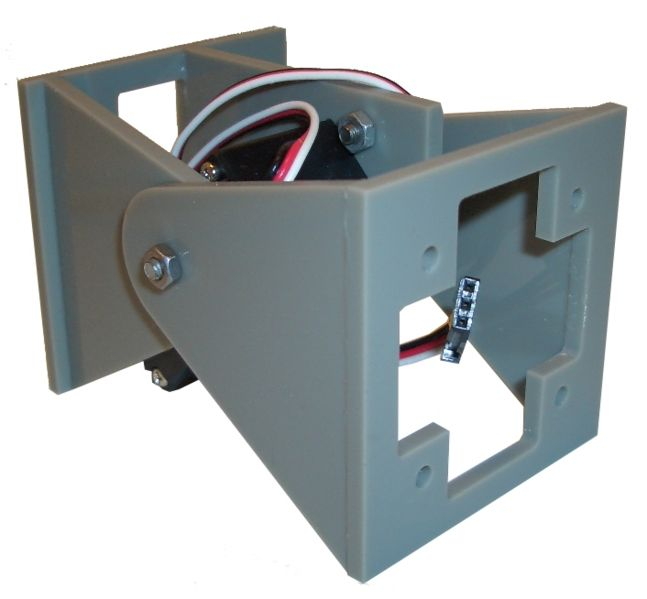
\includegraphics[width=\textwidth]{images/Y1_01.jpg}
                \caption{Y1}
                \label{fig:hardware_y1_mod}
        \end{subfigure}
        ~
        \begin{subfigure}[b]{0.3\textwidth}
                \centering
                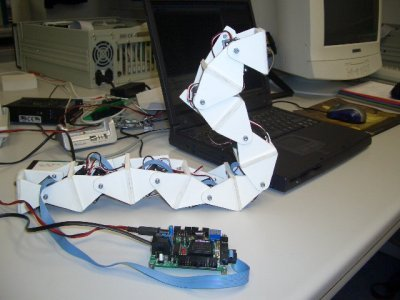
\includegraphics[width=\textwidth]{images/State_art_Y1_cube.jpeg}
                \caption{Cube Revolutions (Y1 snake)}
                \label{fig:hardware_y1_cube}
        \end{subfigure}
        \caption{Module Y1} \label{fig:hardware_y1}
\end{figure}

\newpage
\subsubsection{Y1 module derivatives: MY1 and REPY1}
\label{hardware_repy1}

Based on the Y1 design, Gonzalez-Gomez developed other modules: the MY1 and the REPY-1. The MY1\cite{gonzalez-gomez_website:my1} is a metal version of the Y1 module, manufactured from 2mm thick aluminium with a similar shape to the Y1, and compatible with it. A battery holder and a control board were designed for this module, therefore allowing untethered operation of the robots constructed with this module.\\

The advantages of the MY1 module are a stronger frame, and the incorporation of the control board and power in the robot structure, requiring only either a serial connection with the computer to be controlled, or having the movements loaded on the controller board. This advantages, however, imply a higher cost and a more complicated manufacturing process, increasing the price of the modules.\\

The REPY-1\cite{gonzalez-gomez_website:repy1} module (REPlicable Y1) is a version of the Y1 designed to be printed in a low cost 3D printer, like a RepRap\cite{jones_reprap_2011}. This simplifies the assembly of the module, as it reduces the number of parts to 2, which can be produced at a low price. If printed on a RepRap 3D printer such as a Prusa Medel 3 model, that costs around 300\euro, the filament material to print both module halves costs no more than 1-2\euro.\\

Apart from the reduced cost and even further simplification of the assembly process, the REPY-1 module has other advantages with respect to the Y1 module. Since the 3D printing process does not imply high fixed manufacturing costs (such as material handling costs, set-up costs, mainteinance costs, etc) there is no need to produce a large batch of modules. Instead, modules can be printed one by one as they are needed. This also allows a faster and cheaper prototyping and improvement process, as modules can be produced, assembled and tested in a short period of time at a low price. Improvements can be done to them, and a new batch of the next iteration of prototypes can be manufactured in a short time and at a low cost, achieving a evolution in the design that previously was only possible to be done in software products.\\

\begin{figure}[h]
		\centering
        \begin{subfigure}[b]{0.3\textwidth}
                \centering
                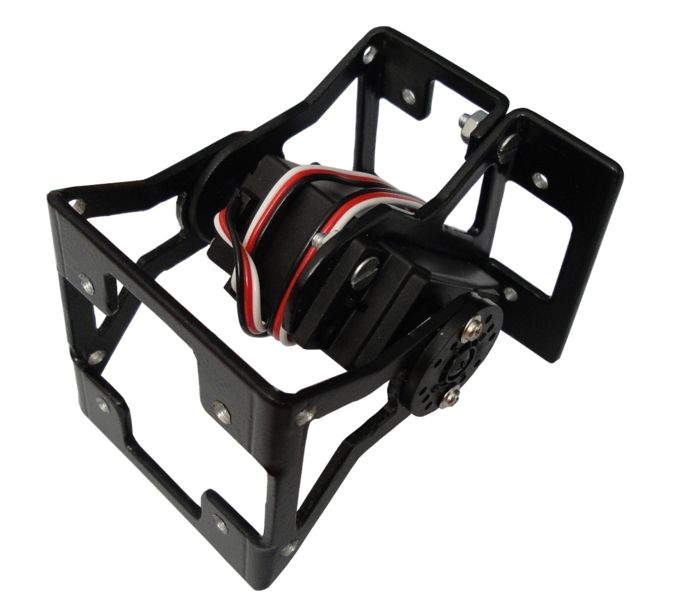
\includegraphics[width=\textwidth]{images/Y1_MY1_01.jpg}
                \caption{MY1}
                \label{fig:hardware_my1}
        \end{subfigure}
        ~
        \begin{subfigure}[b]{0.3\textwidth}
                \centering
                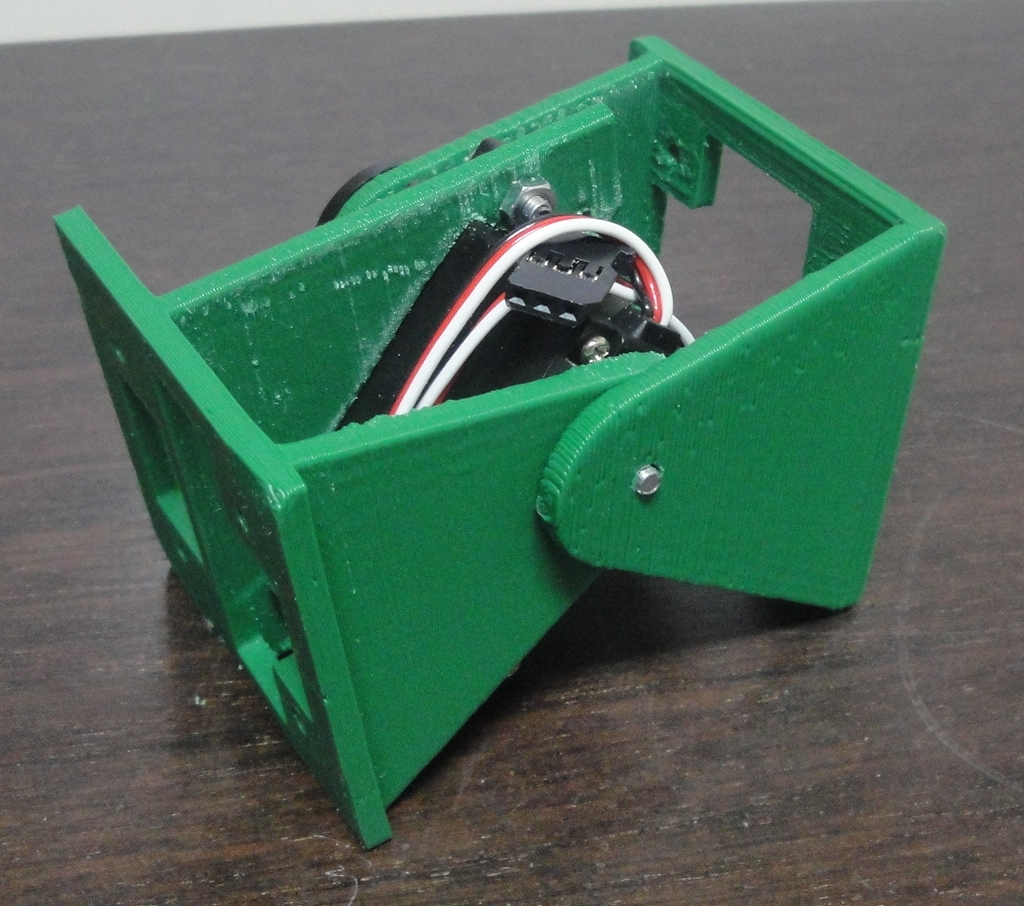
\includegraphics[width=\textwidth]{images/Y1_REPY1_01.jpg}
                \caption{REPY-1}
                \label{fig:hardware_repy1}
        \end{subfigure}
        \caption{Module Y1 derivatives: MY1 and REPY-1} \label{fig:hardware_y1_derivatives}
\end{figure}

The MY1 and REPY-1 modules are also open source, and the files to manufacture them are available in Gonzalez-Gomez's website, with assembly and usage instructions. Having the files publicly available allowed us to download them and print a small batch of 4 REPY-1 modules in order to test them and evaluate their virtues and flaws, in order to improve the design later. We will discuss those improvements made to the original Y1 design on the next section about our design, the REPY-2 module.\\

%%%%%%%%%%%%%%%%%%% REPY-2.x %%%%%%%%%%%%%%%%%%%%%%%%%%%%%%%%%%%%%%%%%%%%
\newpage
\subsection{REPY-2}
\label{hardware_repy-2.x}

Several REPY-1 modules were printed and analyzed on different configurations in order to find if they could be used in this project. After testing them, we realized that the design was a good starting point, but it needed to be improved in order to be used for this thesis.\\

Based on our analysis and tests of the printed version of the Y1 module, the REPY-1 module, we observed the following problems in the module design:

\begin{itemize}
	\item The design was difficult to print correctly and it was very fragile. The part that holds the hobby servo was connected to the rest of the body of the module by a small section that broke while it was being printed, and one of the ears of the module was too thin, so it usually broke when assembling both halves together. 
	
	\item The REPY-1 was designed on OpenSCAD, but it imported the DXF files of the laser-cut Y1 module, extruded them and placed them together, so the module was not parametric. This means that this design only works with the Futaba 3003s hobby servo and the Skycube/Skymega board. This design is therefore not easy to modify or adapt to other hardware different from the original one.
	
	\item The module REPY-1, as well as the module Y1 are not symmetric, since they have the hobby servo placed at an angle of approximately 45º with respect to the base. This results in a more compact module, but allows locomotion of robots only when placed over one of their sides, the opposite one has a straight spine that contains the servo and makes the gait unstable.
	  
	\item Only 2 connectors are present on the Y1 modules and their derivatives, on the front and the back of the module, so the possible configurations that can be assembled with them are restricted to chain-type, 1D configurations. This makes them only suitable for testing locomotion in apodal robots, such as snake robots.
	  
\end{itemize}

Other improvements, such as an active connector to enable self-reconfiguration, or a control board and power management system integrated on each of the modules were also desirable, but discarded due to the temporal and economic constraints of this project.

\subsubsection{First version: REPY-2.0}
We started the design of the module in OpenSCAD, but soon we moved to OOML, since the C++ language allowed us to perform more powerful operations with a clearer syntax. Designing the module with the OOML library instead of directly on OpenSCAD also allowed us to organize the code better, helped by the use of C++ classes.\\

This first version, called REPY-2.0, solved most of the issues found on the original REPY-1 module. The module was designed not just parametric, but object-oriented. This means that a \emph{BasicServo} class and a \emph{BasicPCB} class exist, containing all the dimensions that define the hobby servo and the control board. Instances of these classes are passed to the constructor of the \emph{REPY\_module} class, that uses the stored dimensions to generate automatically a module suitable for being used with that servo and control board. If one wants to build the module with a different model of hobby servo, or with a different control board, he just has to define new servos or PCBs, by inheriting the basic interface from the \emph{BasicServo} and \emph{BasicPCB} classes. If the \emph{REPY\_module} constructor is called with these new servos or PCBs, it will automatically generate a module to be used with them.\\

The module was made symmetrical by placing the hobby servo at a 90º angle with respect to the base of the module, allowing a smooth movement of the module on either of its opposing sides, solving the instablity problem of the Y1 module when placed over the straight side of the module body.\\

The overall design was reinforced so that it was easier to print and stronger, being less likely to break it when assembling the module. The thickness of the walls was increased as thin walls were a frequent cause of failure when printing the REPY-1 module and they broke easily. This thicker walls also allowed the horn of the servo to be embedded in the module upper part,  eliminating the need of using screws to fix the servo horn to the module.\\

This module version was printed for the Futaba 3003s servo with a Skymega board and, in order to test that this design could also generate modules to use with other servos and boards, we also print a smaller version of the module to assemble with the smaller Towerpro SG90 servo, and a small, custom board. Figure \ref{fig:hardware_repy2_big_and_small} shows the two kinds of REPY-2.0 modules printed to test the design. It is important that both modules were generated from the same code, only changing the servo and board objects passed to the module constructor.\\

\begin{figure}[H]
		\centering
        \begin{subfigure}[b]{0.45\textwidth}
                \centering
                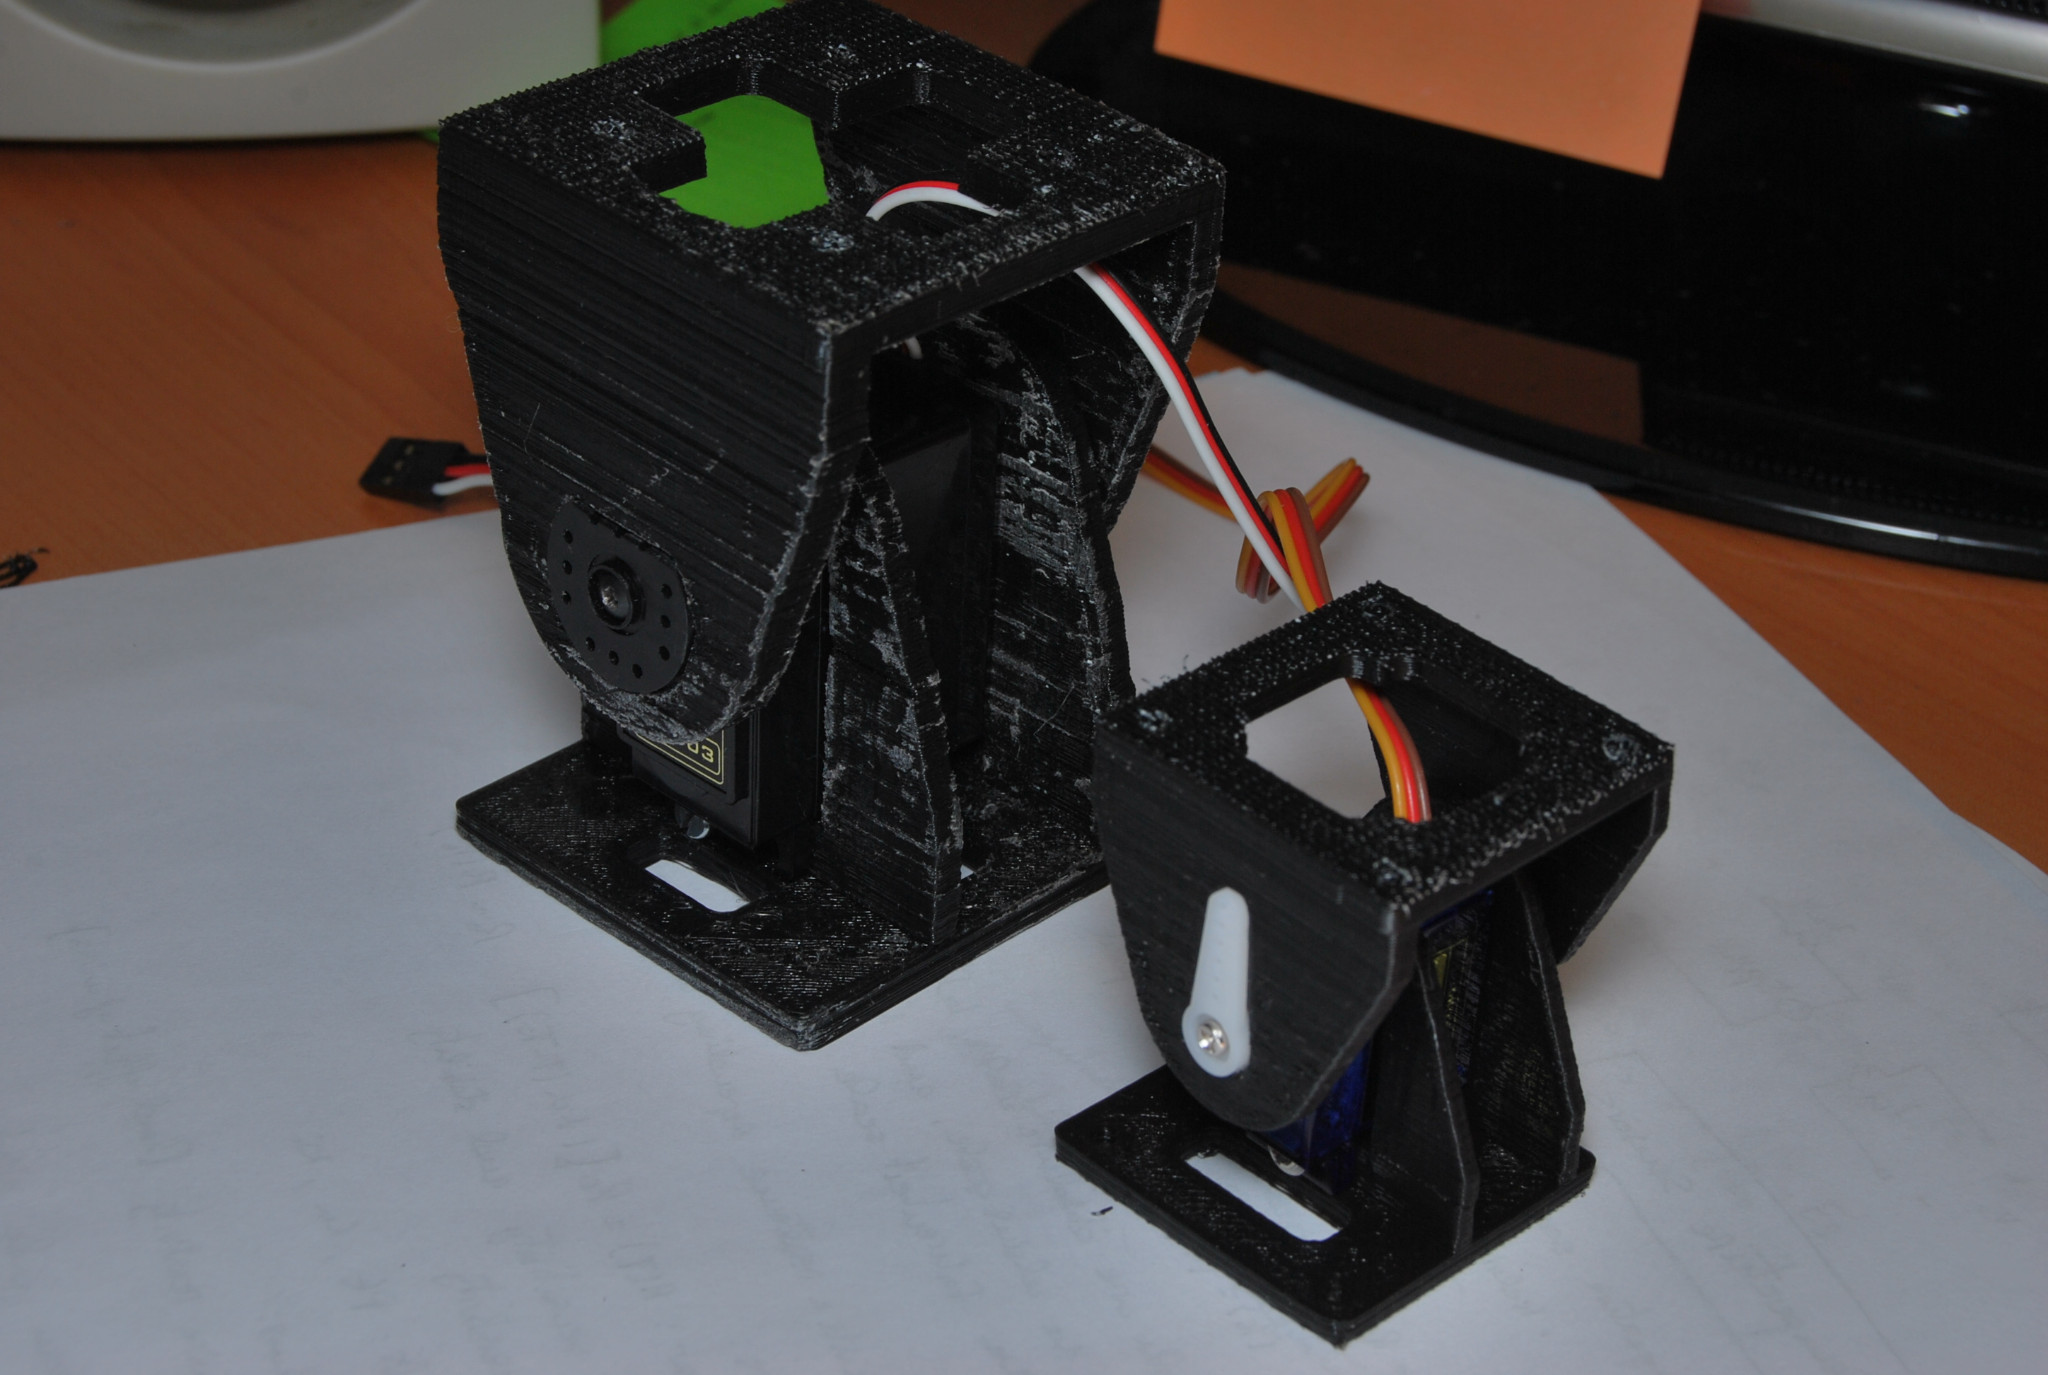
\includegraphics[width=\textwidth]{images/Hardware_repy2_big_and_small_01.jpg}
                \label{fig:hardware_repy2_big_and_small_01}
        \end{subfigure}
        ~
        \begin{subfigure}[b]{0.45\textwidth}
                \centering
                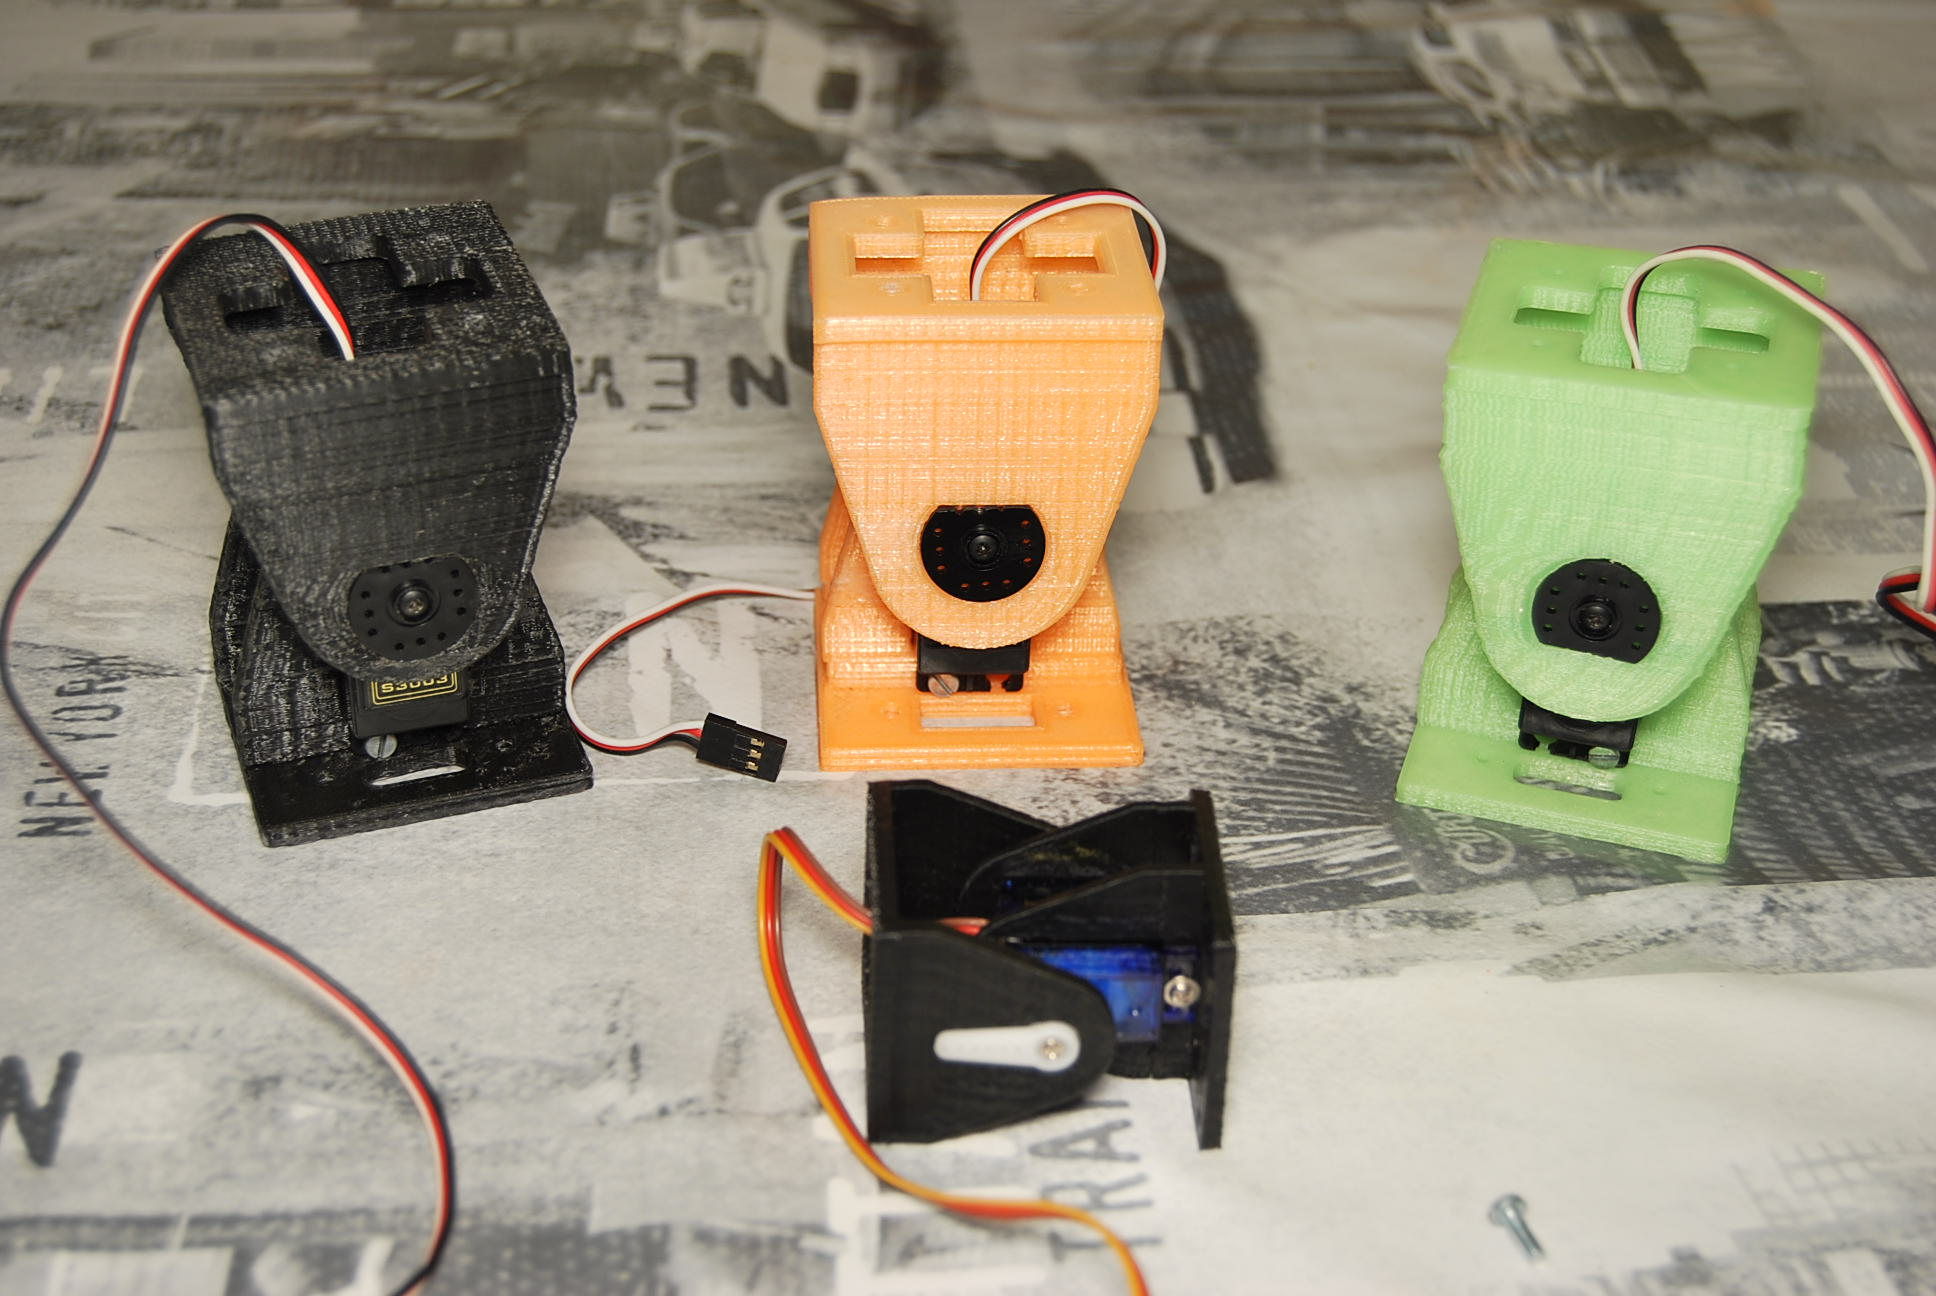
\includegraphics[width=\textwidth]{images/Hardware_repy2_big_and_small_02.jpg}
                \label{fig:hardware_repy2_big_and_small_02}
        \end{subfigure}
        \caption{Two different REPY-2.0 modules for different servos generated from the same code. } \label{fig:hardware_repy2_big_and_small}
\end{figure}


\subsubsection{Second version: REPY-2.1}

A second version of the REPY-2 modules was developed shortly after testing and validating the first version. This version is mostly equal to the first version, but the tolerances for the different fittings are better adjusted. The last of the required improvements, two side connectors for enabling 2D configurations were also added in this version. These connectors are just 4 holes in the same disposition than the holes in the front and back of the module, that allow the connection with other modules with screws, as the front and back connectors did.\\

Since both versions are compatible (in both connector and dimensions), and the main difference is the presence of two extra side connectors, both versions were used to assemble the modular robots to test the locomotion gaits, using the second version ones for the places were a 2D connection between modules were used. This way we could use the first version modules already printed to reduce the number of required modules of the second version.\\

\begin{figure}[H]
		\centering
        \begin{subfigure}[b]{0.4\textwidth}
                \centering
                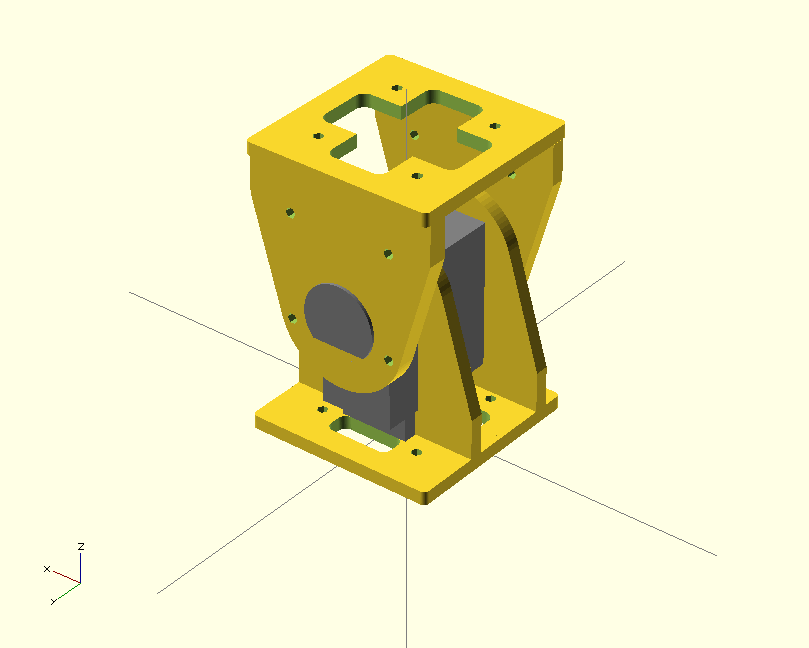
\includegraphics[width=\textwidth]{images/Gait_osc_center_90.png}
                \caption{OpenSCAD render of REPY-2.1 module.}
                \label{fig:hardware_repy2_1_render}
        \end{subfigure}
        ~
        \begin{subfigure}[b]{0.32\textwidth}
                \centering
                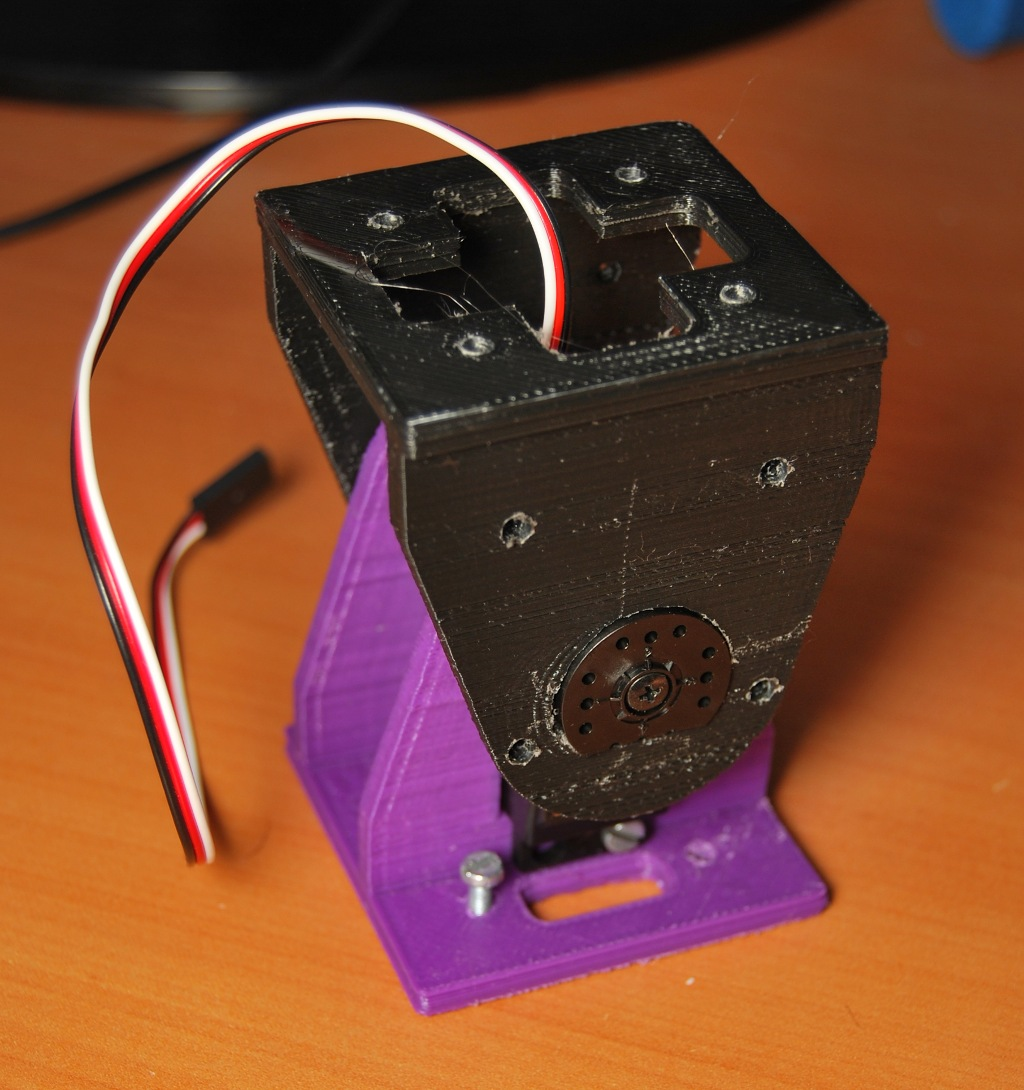
\includegraphics[width=\textwidth]{images/Hardware_REPY_2_1_real.jpg}
                \caption{Printed REPY-2.1 module.}
                \label{fig:hardware_repy2_1_real}
        \end{subfigure}
        \caption{REPY-2.1 modules.} \label{fig:hardware_repy2_1}
\end{figure}


%%%%%%%%%%%%%%%%%%%%%%%%%% Code Structure %%%%%%%%%%%%%%%%%%%%%%%%%%%%%%%%%%%%%%%%%%%%%%%%%%%%%%%%%%%%%%%%%%%%
\subsection{REPY-2.1 OOML code structure}
\label{hardware_ooml_structure}

\begin{figure}[h]
		\centering
        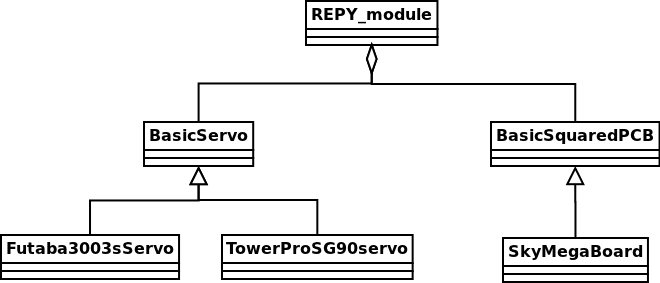
\includegraphics[width=0.7\textwidth]{images/REPY2_class_diagram_main.png}
        \caption{Main class diagram}
        \label{fig:hardware_class_diagram_main}
\end{figure} 


The OOML code for describing the REPY-2 module has a main class, called \emph{REPY\_module}, that defines the geometry of the whole module (both upper and lower parts). This class takes as arguments a servo object that follows the \emph{BasicServo} abstract interface and a PCB object that implements the \emph{BasicSquaredPCB} abstract interface. From this objects the \emph{REPY\_module} extracts the key dimensions and uses them to calculate its own dimensions and geometry automatically. The main class diagram for the module OOML code is shown in figure \ref{fig:hardware_class_diagram_main}.\\

This section will explain the main classes used to model the REPY-2 module with the OOML. More detailed information about the code, useful for developers interested in understanding the code and contribute to the project with new servos, boards or improvements can be found documented online on \url{http://www.dsquaredrobotics.com/wiki/doku.php?id=en:repy-2.0} .\\

The code of the REPY-2 module is open source, and can be found in the following repository: \url{https://github.com/David-Estevez/REPY-2.0} .

\subsubsection{Class REPY\_module}

\begin{figure}[h]
		\centering
        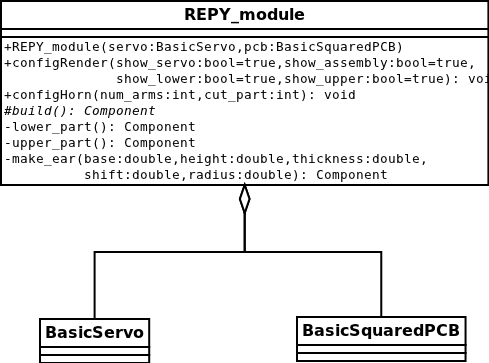
\includegraphics[width=0.5\textwidth]{images/REPY2_class_diagram_REPY_module.png}
        \caption{Class diagram for REPY\_module}
        \label{fig:hardware_class_diagram_REPY_module}
\end{figure} 

The class \emph{REPY\_module} generates the geometry of the module. It extracts the required dimensions from a \emph{BasicServo} and a \emph{BasicSquaredPCB} and calculates its own dimensions from them.\\

With the function \emph{configRender()} the user can specify if the OpenSCAD code generated from this OOML component will represent the upper part of the module, the lower part of the module or both, apart from other options as if those parts will be shown in an assembly view or in a position ready to be printed as well as if the servo will be shown or no. It is also possible to select the servo horn to be used between the ones available for each servo with the function \emph{configHorn}.\\

The upper and lower part are defined in different private functions, \emph{lower\_part()} and \emph{upper\_part()}, that are called by the function \emph{build()}, which generates the whole model depending on the configuration parameters selected. As both parts of the module use a similar shape for their sides, a function \emph{make\_ear()} is defined to create them easily.\\


\subsubsection{Class BasicSquaredPCB}
\begin{figure}[h]
		\centering
        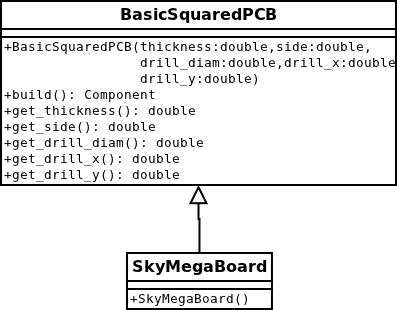
\includegraphics[width=0.5\textwidth]{images/REPY2_class_diagram_BasicSquaredPCB.png}
        \caption{Class diagram for BasicSquaredPCB}
        \label{fig:hardware_class_diagram_BasicSquaredPCB}
\end{figure} 

The class \emph{BasicSquaredPCB} represents a simple squared PCB with four holes for placing screws to attach it to the module. It is defined by the length of the side, the thickness of the PCB, and the location and radius of the drills for the screws.\\

The SkyMega board dimensions are included in the \emph{SkyMegaBoard}, that is used to create the standard size module. For the small module, a custom board was defined using the constructor of the \emph{BasicSquaredPCB}  class.\\


\subsubsection{Class BasicServo}

Hobby servos can be created using as a base the \emph{BasicServo} class. The main dimensions of the servo are included in this class, and can be accessed with the getter functions. This way the \emph{REPY\_module} class can extract the main dimensions of the servo to calculate its own dimensions. The class diagram of figure \ref{fig:hardware_class_diagram_BasicServo} shows the getter functions available to request the servo dimensions.\\

\begin{figure}[h]
		\centering
        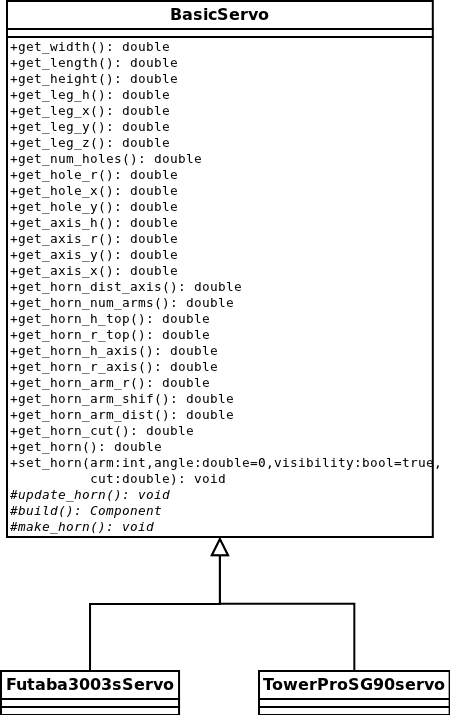
\includegraphics[width=0.5\textwidth]{images/REPY2_class_diagram_BasicServo.png}
        \caption{Class diagram for BasicServo}
        \label{fig:hardware_class_diagram_BasicServo}
\end{figure} 

Different horns can be defined for a servo, and selected with the \emph{set\_horn()} function. This horn is later created on the \emph{build()} method using the \emph{make\_horn()} with the rest of the module.\\

Two different servos were defined, the \emph{Futaba3003sServo} for the standard size module and the \emph{TowerProSG90Servo} for the smaller one. These classes contain the dimensions of the Futaba 3003s servo and the Tower Pro SG90 servo respectively, as well as some horns with different number of arms for each one.\\

\newpage
\subsection{Building the REPY-2.1 module}
\label{hardware_assembly}
In this section we will explain how to build and assemble a REPY-2.1 module. The files required for manufacturing the two parts that compose the module can be downloaded from the internet, as we are making them publicly available with an open source license.

\subsubsection{Generating the 3D files}

The first step to build the REPY-2 modules is to obtain the STL files in order to print the parts of the module. These files can be downloaded from the module repository: \url{https://github.com/David-Estevez/REPY-2.0} , or compiled from the source code.\\

The requirements for obtaining the files from the sources are the following:
\begin{itemize}
	\item \textbf{CMake.} CMake is used to generate the makefiles used to compile the project C++ code. CMake can be downloaded from \url{http://www.cmake.org/cmake/resources/software.html}. More detailed instructions can be found on section \ref{software_install_cmake}.
	
	\item \textbf{OOML.} The Object Oriented Mechanics Library allow us to generate OpenSCAD code from the C++ code, and can be downloaded from \url{http://iearobotics.com/oomlwiki/doku.php?id=start} . The website counts with very detailed instructions for installing OOML.
	
	\item \textbf{OpenSCAD.} The OOML only generates OpenSCAD code. For obtaining the STL files, OpenSCAD is required. It can be downloaded from its website: \url{http://www.openscad.org/} .\\
\end{itemize}

Once the dependencies are installed, the code has to be built. The instructions for building the code are:
\begin{enumerate}
	\item Edit the file ``CMakeLists.txt'' to include the path to the OOML include directory. For example, in the authors system this path was ``/usr/include/ooml''.

	\item Open a terminal, go to the REPY-2.0 directory and build it using cmake:
        \Bash
		\begin{lstlisting}
	$ mkdir build
	$ cd build
	$ cmake ..
	$ make 
	$ make install
		\end{lstlisting} %$	
Notice that for the installation you won't need to be superuser, as it is installed in a directory called \emph{`bin'} in the \emph{`REPY-2.0 folder'}.

	\item Execute the program \emph{REPY-2.0}, that will create the SCAD files and, optionally, the STL files for the REPY-2.0 module.
	
	\item If the STL files were not generated using the \emph{REPY-2.0} program, open the desired SCAD file with OpenSCAD  and compile it manually.
\end{enumerate}

\newpage
\subsubsection{Printing the parts}

Once the STL files have been downloaded or generated, the next step is printing them on the 3D printer. The concrete steps that are to be followed to print depend on the 3D printer that is going to be used and the software to control it. These low-cost 3D printers used create the object by depositing plastic layer by layer until the object is complete. The plastic used is tipically ABS (Acrylonitrile butadiene styrene) or PLA (Polylactic Acid)\\

The steps required to print the files involve usually to generate the GCODEs (codes that are control the CNC machine, specifying the velocity and position of its tool, in this case, the plastic extruder required to follow the required path, as well as the amount of plastic to extrude in each position) with a slicer software. The slicer software calculates those toolpaths by slicing the 3D models in several planes, and calculating the trajectories required in each layer to form the 3D object.\\

For the module to be assembled two parts need to be printed: the lower part and the upper part. As hobby servos usually come with more than one horns with different geometries available, there are more than one upper parts in the repository, each one to be used with a different type of horn. Only one upper part is needed to build the module, that has to be selected according to the horn to be used.


\subsubsection{Assembling the module}

\noindent
Each module requires the following materials to be built:
\begin{itemize}
	\item 1x Upper part of the module (3D printed part)
	\item 1x Lower part of the module (3D printed part)
	\item 1x Futaba 3003s servo
	\item 1x M3x8mm screw
	\item 4x M3x10mm screws (minimum 2)
	\item 4x M3 nuts (minimum 2)
	\item 4x M3 washers (minimum 2)
\end{itemize}

\newpage

\begin{figure}[H]
		\centering
        \begin{subfigure}[b]{0.46\textwidth}
                \centering
                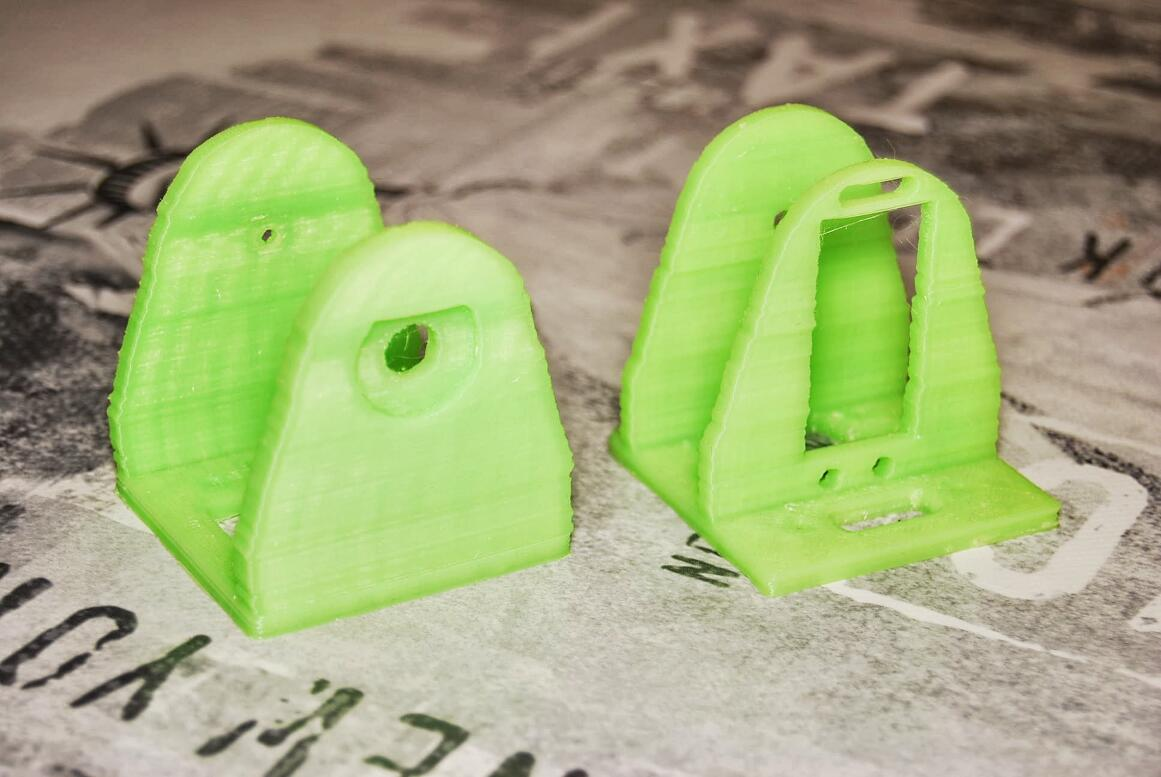
\includegraphics[width=\textwidth]{images/REPY2_assembly_01.jpg}
                \caption{Printed plastic parts needed: upper part and lower part.\\}
                \label{fig:hardware_assembly_01}
        \end{subfigure}
        ~
        \begin{subfigure}[b]{0.46\textwidth}
                \centering
                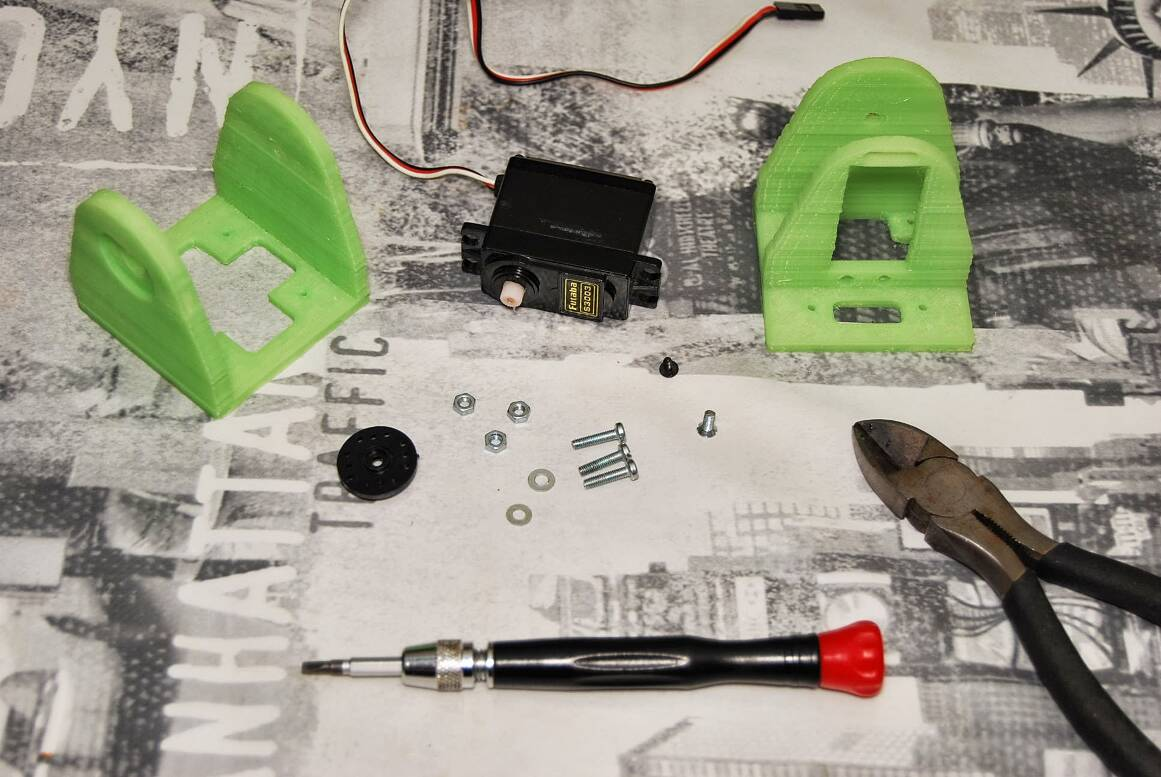
\includegraphics[width=\textwidth]{images/REPY2_assembly_02.jpg}
                \caption{Overview of tools and parts needed for assembling the module.}
                \label{fig:hardware_assembly_02}
        \end{subfigure}
        \caption{Required materials to build the REPY-2.1 module} 
        \label{fig:hardware_assembly_materials}
\end{figure}

\begin{figure}[H]
        \centering
        \begin{subfigure}[b]{0.46\textwidth}
                \centering
                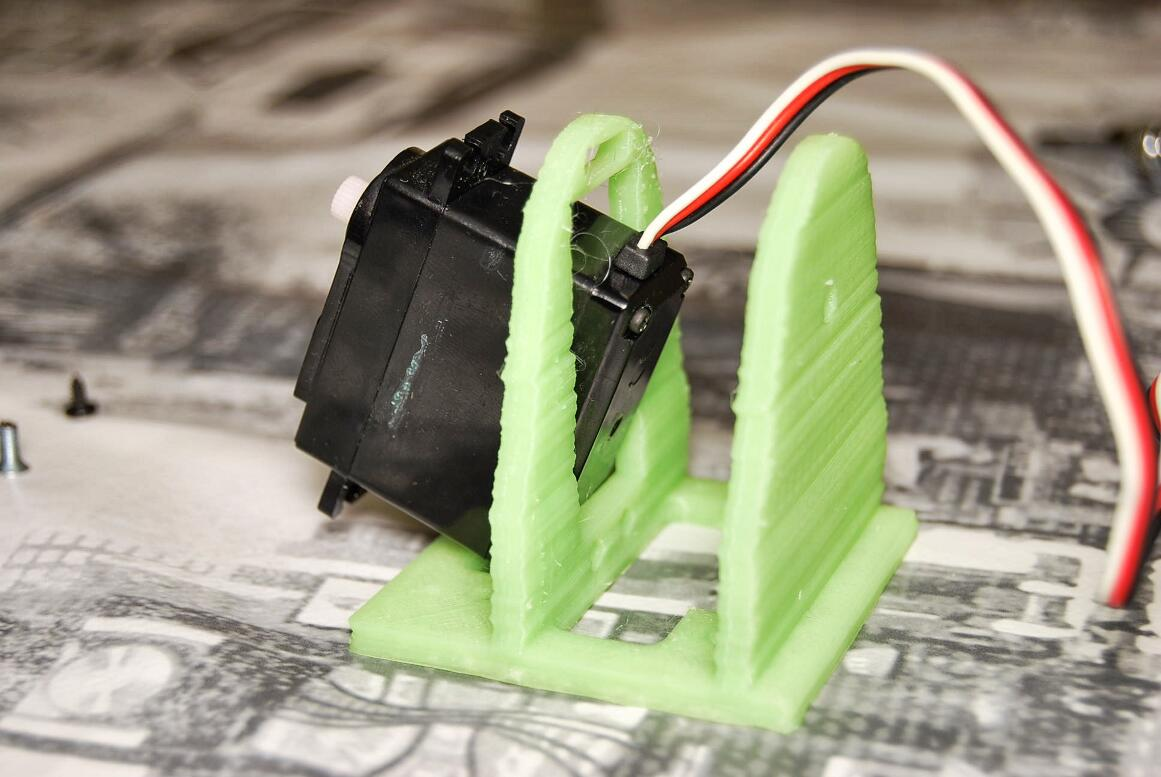
\includegraphics[width=\textwidth]{images/REPY2_assembly_03.jpg}
                \caption{Insert carefully the module in the lower part in the hole prepared to hold the servo.\\}
                \label{fig:hardware_assembly_03}
        \end{subfigure}
        ~
        \begin{subfigure}[b]{0.46\textwidth}
                \centering
                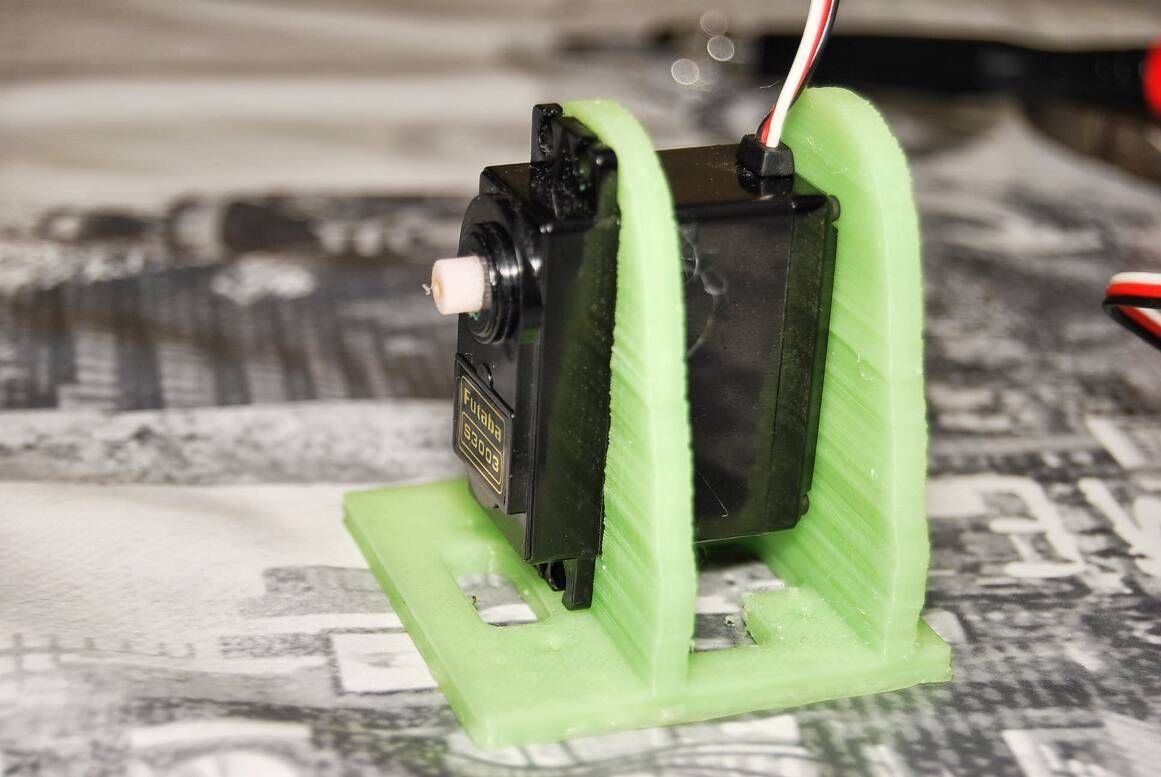
\includegraphics[width=\textwidth]{images/REPY2_assembly_04.jpg}
                \caption{Check that the servo leg holes and the module corresponing holes are aligned.\\}
                \label{fig:hardware_assembly_04}
        \end{subfigure}
        ~
        \begin{subfigure}[b]{0.46\textwidth}
                \centering
                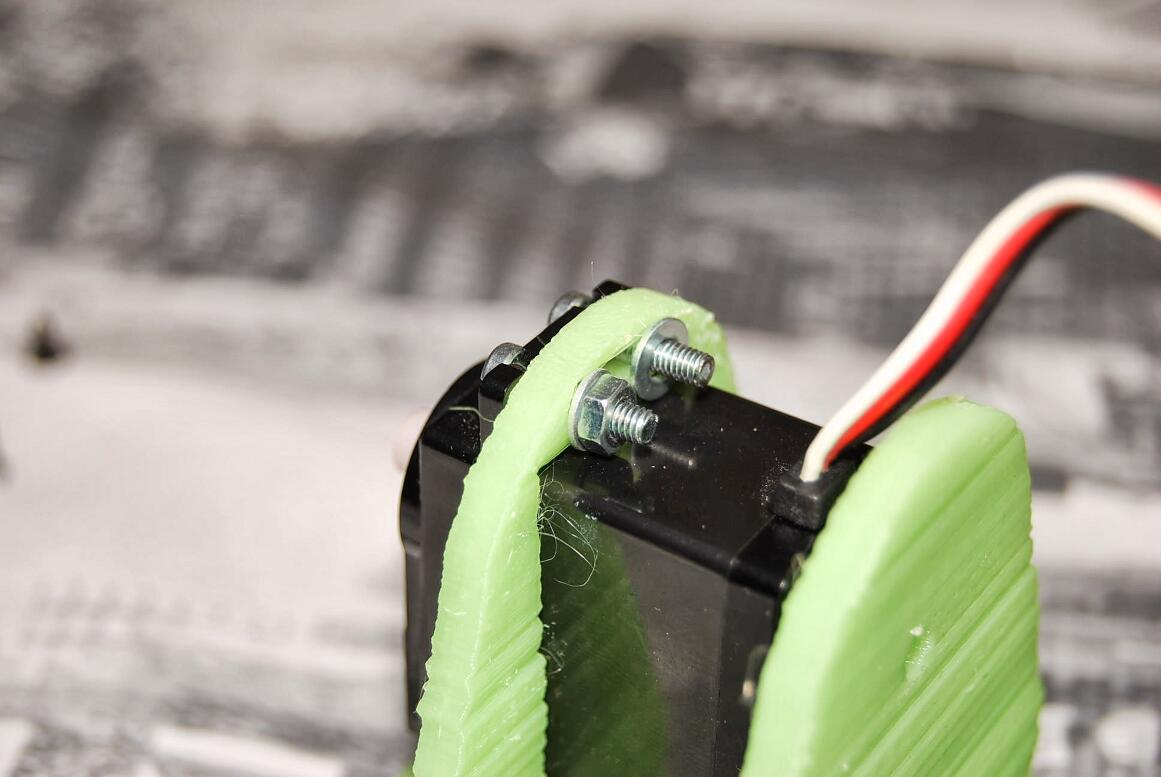
\includegraphics[width=\textwidth]{images/REPY2_assembly_05.jpg}
                \caption{Fix the servo to the module using the screws, nuts and washers for the top holes.\\}
                \label{fig:hardware_assembly_05}
        \end{subfigure}
        ~
        \begin{subfigure}[b]{0.46\textwidth}
                \centering
                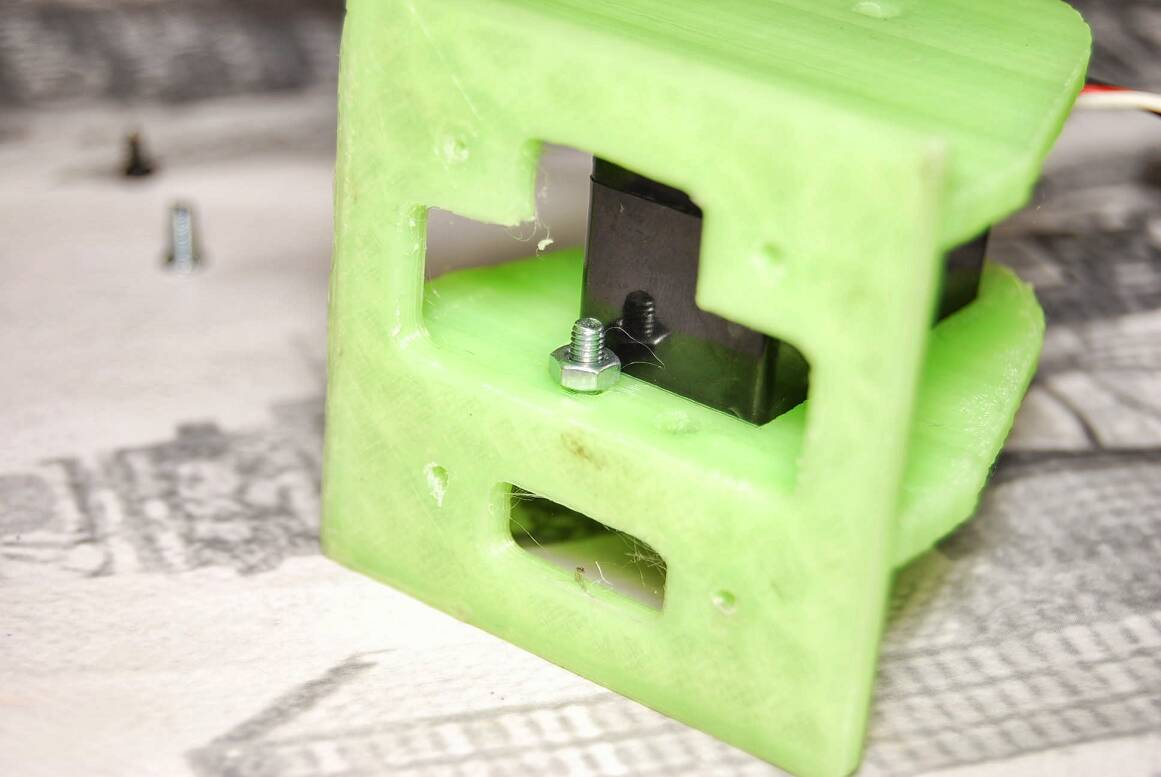
\includegraphics[width=\textwidth]{images/REPY2_assembly_06.jpg}
                \caption{Fix the servo to the module using the screws, nuts and washers for the bottom holes.\\}
                \label{fig:hardware_assembly_06}
        \end{subfigure}
        \caption{Assembly of the lower part} 
        \label{fig:hardware_assembly_lower}
\end{figure}

\begin{figure}[H]
        \centering
        \begin{subfigure}[b]{0.46\textwidth}
                \centering
                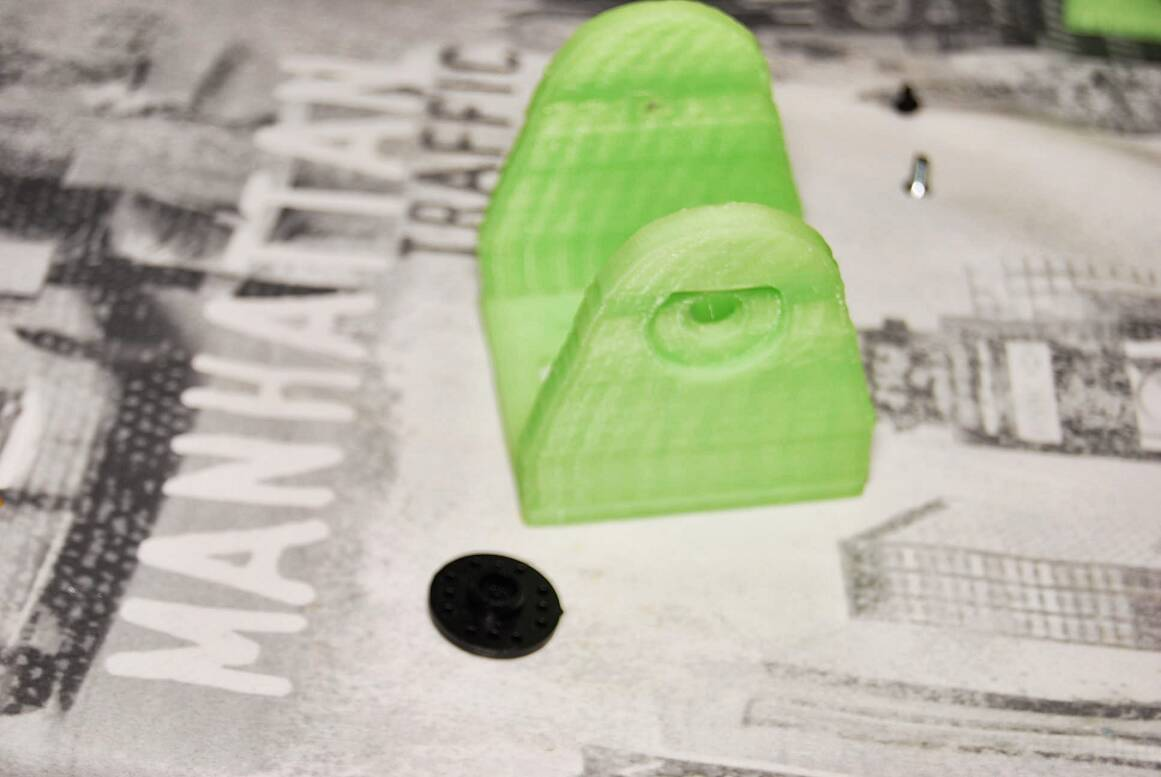
\includegraphics[width=\textwidth]{images/REPY2_assembly_08.jpg}
                \caption{Materials required to assemble the upper part.\\~\\~}
                \label{fig:hardware_assembly_08}
        \end{subfigure}
        ~
        \begin{subfigure}[b]{0.46\textwidth}
                \centering
                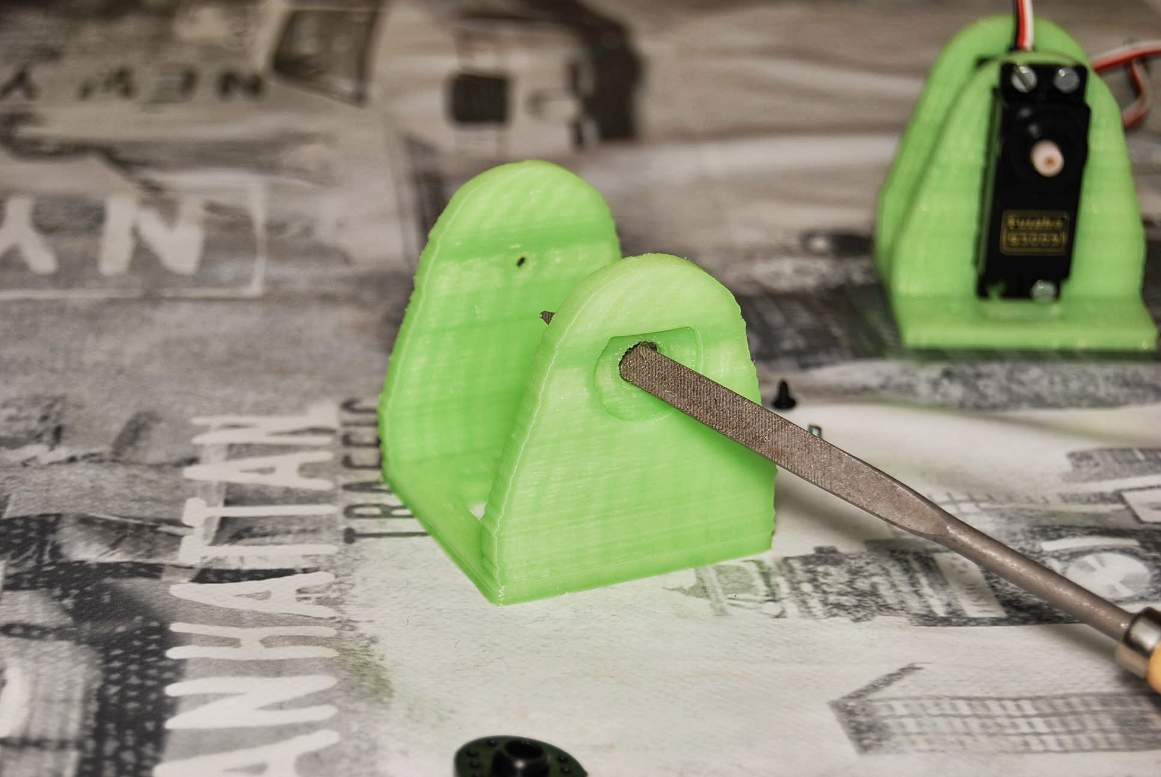
\includegraphics[width=\textwidth]{images/REPY2_assembly_09.jpg}
                \caption{If needed, file the hole until the servo horn fits tightly on it.\\}
                \label{fig:hardware_assembly_09}
        \end{subfigure}
        ~
        \begin{subfigure}[b]{0.46\textwidth}
                \centering
                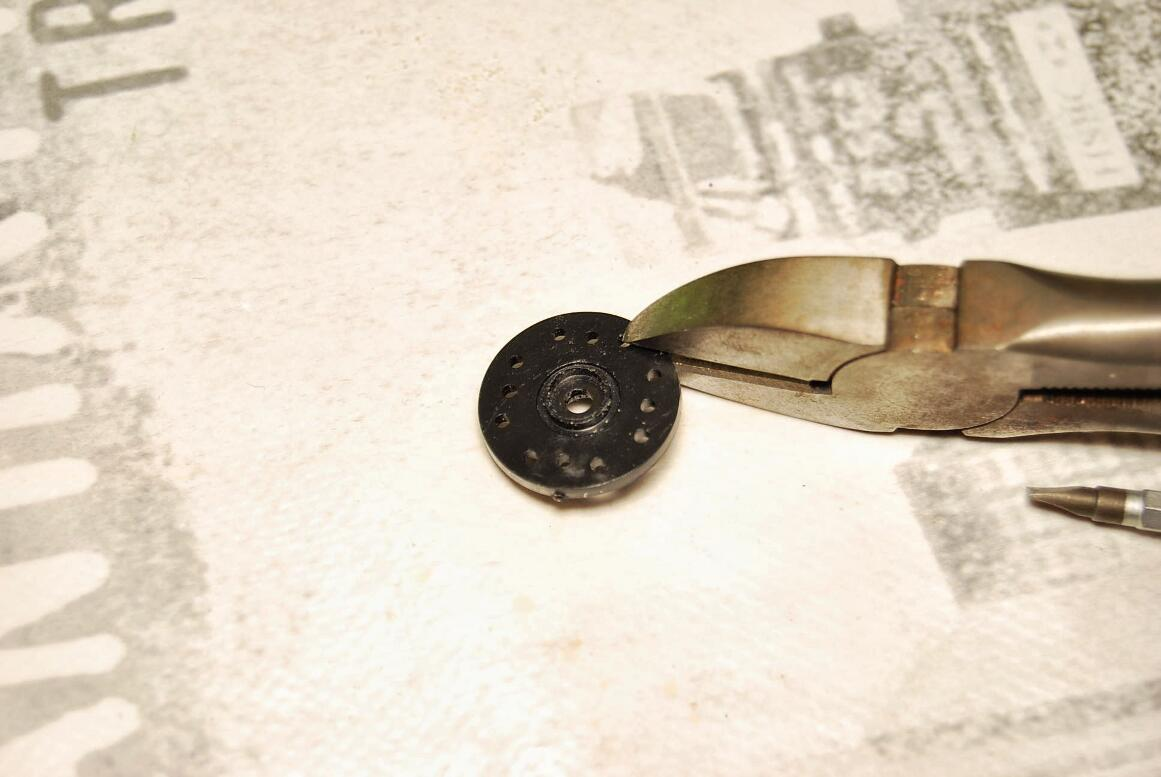
\includegraphics[width=\textwidth]{images/REPY2_assembly_10.jpg}
                \caption{With the help of some cutting pliers, cut the horn with the shape of the corresponding hole in the printed part.\\}
                \label{fig:hardware_assembly_10}
        \end{subfigure}
        ~
        \begin{subfigure}[b]{0.46\textwidth}
                \centering
                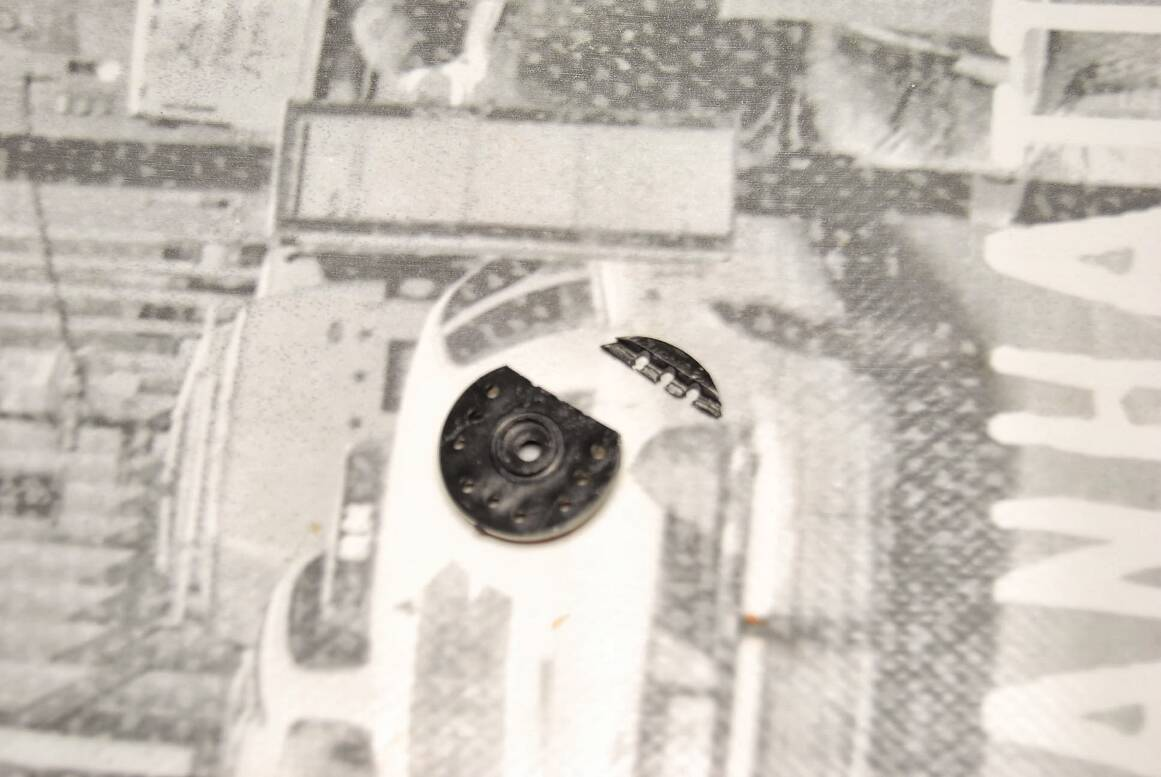
\includegraphics[width=\textwidth]{images/REPY2_assembly_11.jpg}
                \caption{After the cut, the servo horn should look like this.\\~\\~}
                \label{fig:hardware_assembly_11}
        \end{subfigure}
        ~
        \begin{subfigure}[b]{0.46\textwidth}
                \centering
                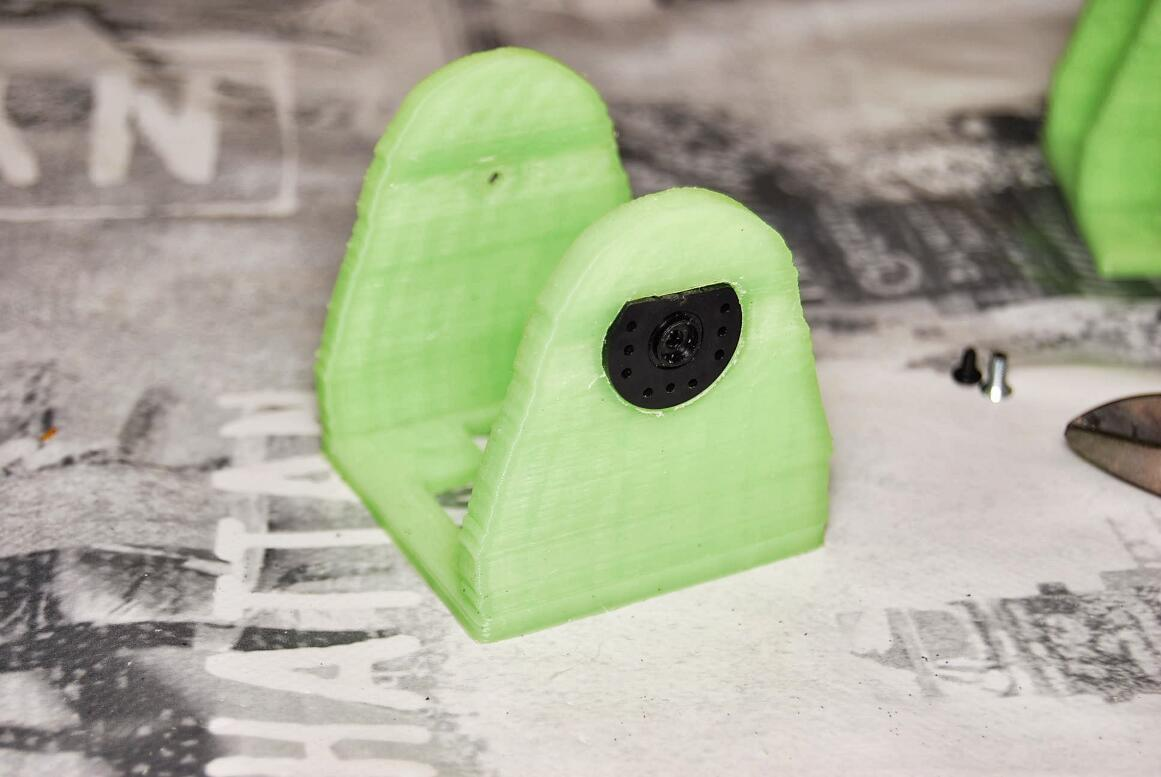
\includegraphics[width=\textwidth]{images/REPY2_assembly_12.jpg}
                \caption{Insert the horn in the corresponding hole of the upper part.\\ }
                \label{fig:hardware_assembly_12}
        \end{subfigure}
        ~
        \begin{subfigure}[b]{0.46\textwidth}
                \centering
                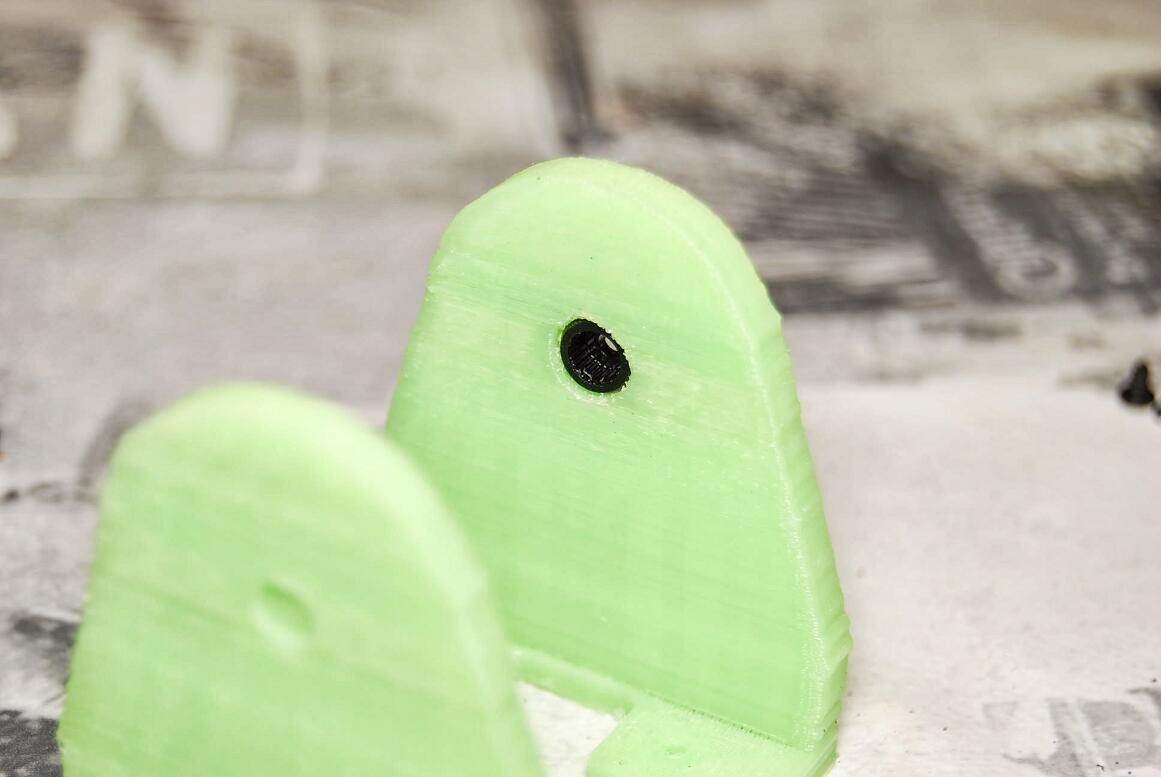
\includegraphics[width=\textwidth]{images/REPY2_assembly_13.jpg}
                \caption{The module should look like this seen from behind after inserting the horn.\\}
                \label{fig:hardware_assembly_13}
        \end{subfigure}
        \caption{Assembly of the servo horn} 
        \label{fig:hardware_assembly_horn}
\end{figure}

\begin{figure}[H]
        \centering
        \begin{subfigure}[b]{0.46\textwidth}
                \centering
                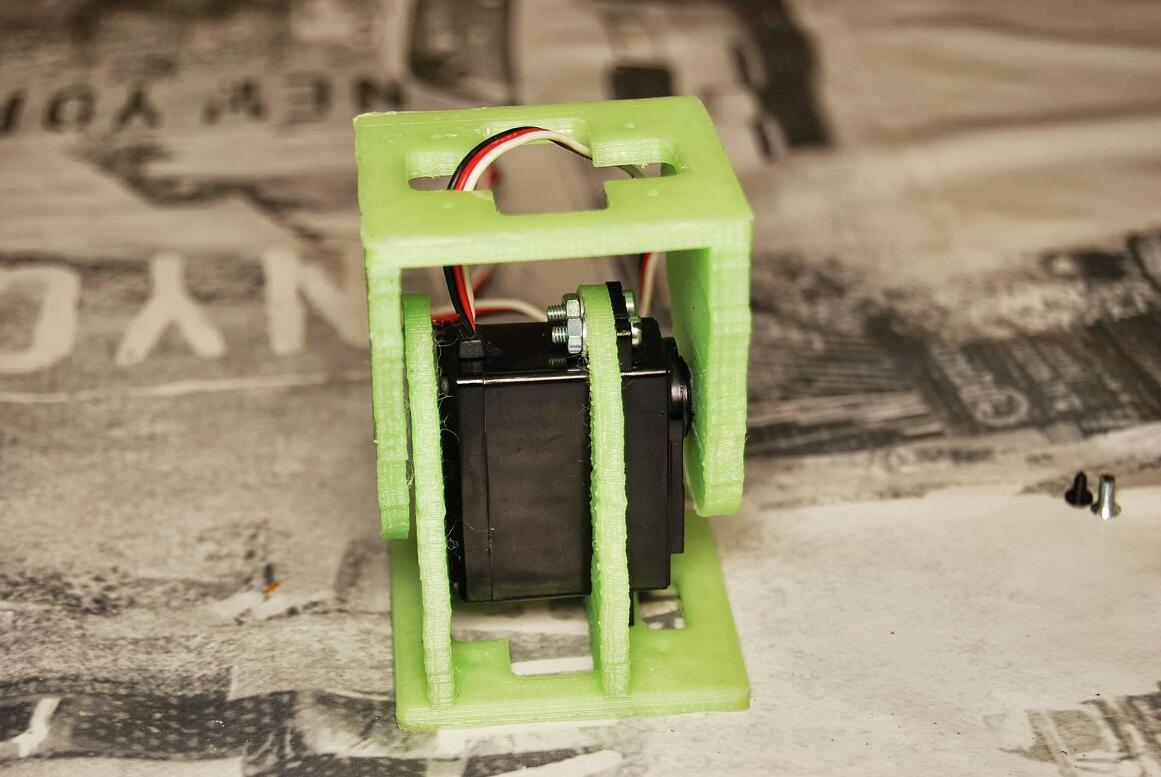
\includegraphics[width=\textwidth]{images/REPY2_assembly_14.jpg}
                \caption{Connect both parts carefully. The servo must be connected to the control board and set to 90º in order to ensure that the 90º position of the servo corresponds to the 90º position of the servo.\\}
                \label{fig:hardware_assembly_14}
        \end{subfigure}
        ~
        \begin{subfigure}[b]{0.46\textwidth}
                \centering
                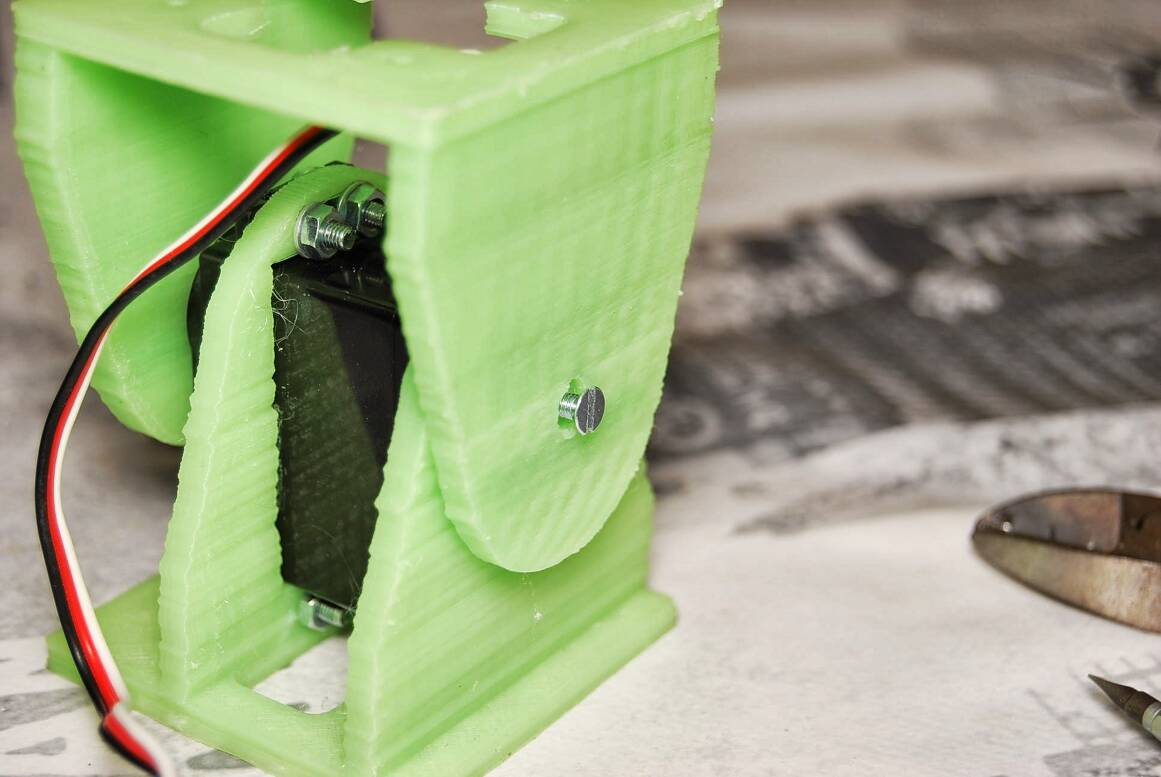
\includegraphics[width=\textwidth]{images/REPY2_assembly_15.jpg}
                \caption{Insert the screw for the fake axis.\\~\\~\\~\\~}
                \label{fig:hardware_assembly_15}
        \end{subfigure}
        ~
        \begin{subfigure}[b]{0.46\textwidth}
                \centering
                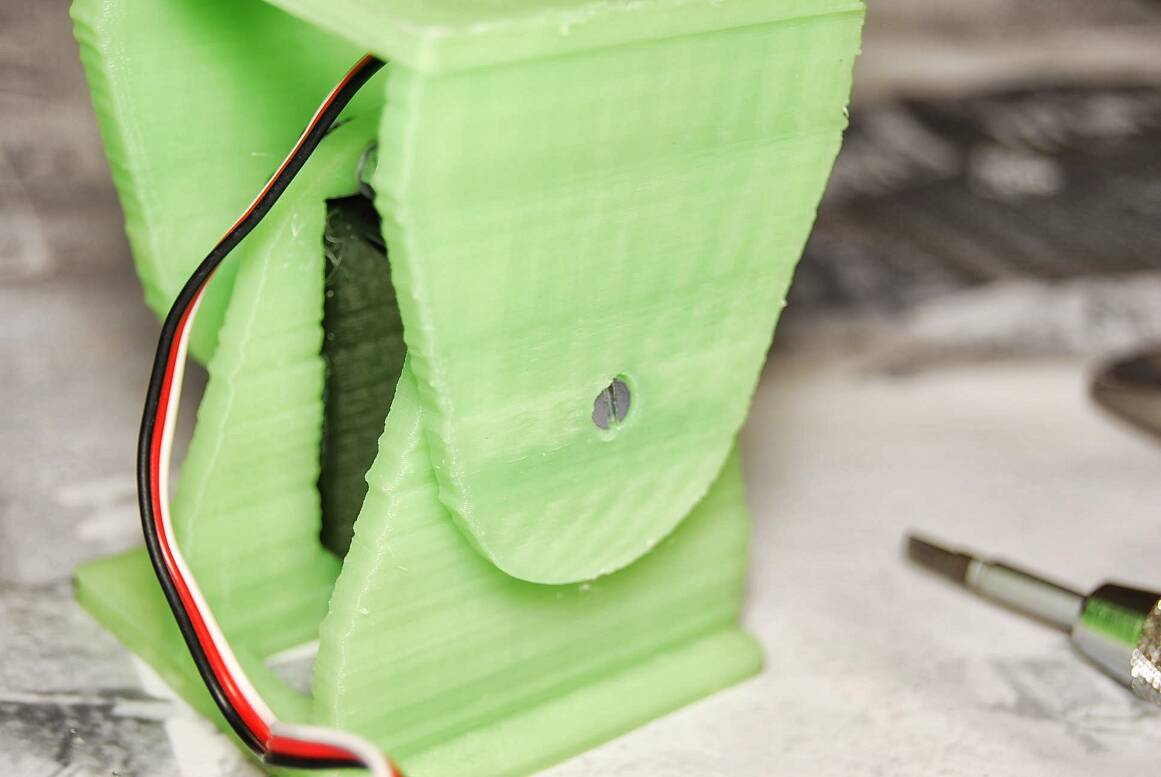
\includegraphics[width=\textwidth]{images/REPY2_assembly_16.jpg}
                \caption{The screw of the fake axis should not protude from the servo body.\\}
                \label{fig:hardware_assembly_16}
        \end{subfigure}
        ~
        \begin{subfigure}[b]{0.46\textwidth}
                \centering
                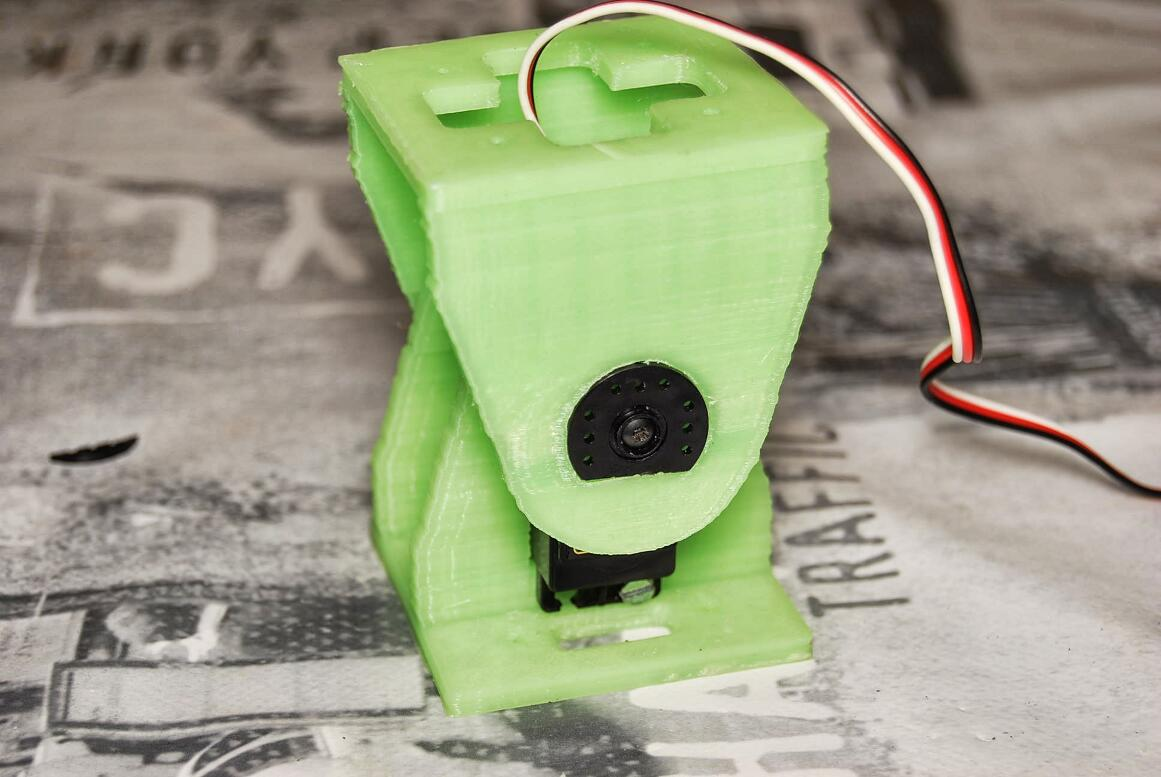
\includegraphics[width=\textwidth]{images/REPY2_assembly_17.jpg}
                \caption{The REPY-2 module is ready to be used!\\~\\~}
                \label{fig:hardware_assembly_17}
        \end{subfigure}
        \caption{Putting together the module} 
        \label{fig:hardware_assembly_module}
\end{figure}

\newpage 

%%%%%%%%%%%%%%%%%%%%%% ELECTRONICS %%%%%%%%%%%%%%%%%%%%%%%%%%%%%%%%%%%%%%%%%%%%
\section{Electronic control board}
\label{hardware_electronics}

For the control of the robot, a controller board was designed. For this we followed the same approach that with the module, using a previous, open source design as a reference for our board, improving and fixing all the flaws we observed on the original board.\\

This section explains the software and platforms used for the design of the board software and firmware. Then, it describes the previous existent boards and the discovered weaknesses of the design. Finally, our board design is presented.


%%%%%%%%%%%%%%%%%%% Tools & software & etc %%%%%%%%%%%%%%%%%%%%%%%%%%%%%%%%%%%%%%%%%%%
\subsection{Software and platforms used}
\label{hardware_electronic_tools}

In this section we will discuss the main software tools and microcontroller platforms used. The modular robot control board, and its firmware, were developed using the Arduino platform and, for the design of our PCB, an open source program called KiCad was employed.

\subsubsection{Arduino}

Arduino \cite{arduino} is an open source electronics prototyping platform originally developed for artists, designers and hobbyists that simplifies working with microcontrolling. It is currently very extended its use in education as a first point of contact with microcontrollers, due to its simplicity.\\

The Arduino platform offers several development boards with different microcontrollers within a wide range of features, that can be selected depending on the project requirements. These boards go from the popular Arduino UNO board, that features an ATmega328, a 8-bit microcontroller with 32KB of flash and 2KB of RAM, to the latest, more advanced boards such as the Arduino DUE, that includes a 32-bit ARM processor running at 84 MHz, with 512 KB of flash and 96 KB of RAM. The schematics and CAD files for these boards are publicly available, which has promoted the appearance of several non-oficial derivative boards, Arduino-compatible, designed for concrete tasks, such as the Ardupilot, a board to control Unmanned Aerial Vehicles or the Skymega, a board for modular robotics, that will be discussed in a later section.\\

As the Arduino platform has defined a standard physical format for their development boards, some extension boards have appeared, called ``shields'', that are plugged in the development board, adding extra hardware to the Arduino boards, such as H-bridges for controlling motors or wireless transceivers for communication with other devices.\\

The principal aspects that make the Arduino easy to use are mainly two. The first one is that this platform is not limited to the hardware, but it also counts with an Integrated Development Environment (IDE) to develop the firmware to be programmed on the microcontroller and manage the board, as well as several libraries to control the microcontroller peripherals and other hardware easily. Most of these libraries have been developed by the community of Arduino users, that have published them with open source licenses for the benefit of all the Arduino community.\\

The second one is the bootloader for the Arduino boards, that allows the microcontroller to be programmed over a serial connection, and removes the necessity of a external programmer to load the firmware to the microcontroller. The process of compiling the code is also simplified by integrating the compiler toolchain into the Arduino IDE.\\

The Arduino platform has been selected over other alternatives, such as using microcontrollers from other vendors like Microchip or STMicrocontrollers because of the following reasons:

\begin{itemize}
	\item Extensive documentation and code examples can be found online due to the openness and popularity of the platform.
	
	\item The Arduino libraries reduce the development time by offering a high-level interface to the basic and advanced features of the microcontroller.
	
	\item The availability of the schematics and CAD files allows us to develop a compatible board that adapts to our requirements based on a existent and tested design, that ensures us that the hardware will work without problems, and reduces the development time.
	
	\item All this tools can be downloaded for free from the Arduino website, as opposed to other propietary IDEs, reducing the cost of the project, as no money has to be spent on development tools. 
\end{itemize}


\subsubsection{KiCad EDA Software Suite}

KiCad \cite{kicad:website} is a multiplatform, open source software suite for Electronic Design Automation (EDA). It was started by Jean-Pierre Charras, a French researcher in the field of electrical engineering, and it is composed of four main programs that perform the different functions required for the design of electronic circuits:\\

\begin{itemize}
	\item \textbf{Eeschema:} Schematic editor. This is the first step in the KiCad workflow, the creation of a schematic detailing the circuit components and connections. 
		\item \textbf{Cvpcb:} Footprint selector for components association. Once the schematic is finished, the netlist containing all the connections is generated, and the component footprints are selected from the libraries with this program.
	\item \textbf{Pcbnew:} Printed circuit board editor. After assigning the footprints to the components, the footprints and netlist are loaded in the PCB editor to make the board layout and routing. Once the PCB is designed, the GERBER files can be generated in order to manufacture the PCB.
	\item \textbf{Gerbview:} GERBER file viewer. With this program the GERBER files can be opened and inspected to check that they are correct before sending them to the manufacturer.

\end{itemize} 

For the design of the PCB in charge of the control of the robot, KiCad was used. Apart from the fact that this program is free, so no cost related to software licences was incurred, KiCad was chosen over other alternatives due to its ease of use and simplicity. Other factors that influenced the decision were that the author had previous experience with this software and the absence of limitations, such as PCB size, number of layers, etc.

%%%%%%%%%%%%%%%%%%% Previous work %%%%%%%%%%%%%%%%%%%%%%%%%%%%%%%%%%%%%%%%%%%%
\subsection{Previous work}
\label{hardware_electronics_previouswork}

For the control of the modular robots built from Y1 modules some boards already existed. Instead of designing a new board from scratch, and as the schematics of those boards were available due to them being open source, they were used as reference to design our board. As we had already worked previously with the boards in other projects, we knew the limitations of the boards to be solved in our design. The improvements added, as well as a decription of the existing boards is presented in this section.\\

\subsubsection{Skycube}
\label{hardware_skycube}

The Skycube \cite{gonzalez-gomez_website:skycube} is a board designed by Gonzalez-Gomez for controlling modular robots, featuring a PIC16F876A microcontroller running at 20MHz. It is compatible with the Y1 modules (and derivatives) and, as them, its schematics and CAD files have been released publicly with a open source license.\\

It allows the control of up to 8 hobby servos, with 4 connectors on each face to make their connection easier. Power and I2C communication connectors are also placed on both faces to allow connections on both sides of the board. The I2C bus can be used for communication between Skycube boards. The board also has a ICSP (In-Circuit Serial Programming) connector for burning the firmware with a programmer, and a connector breaking out the serial pins TX and RX, which is useful for serial communications and to upload firmware using a bootloader.\\

Even though the board counts with a connector for setting a I2C communication bus, the board is intended as a central controller for the whole modular robot, as the I2C is not a multimaster bus, and its length is limited by the capacitance of the transmission lines, as it was designed as a bus for communication between different integrated circuits inside the PCB.\\

A LED and a push button are present in the board, and can be used to interact with the program, supplying a simplistic input and output interface with the user. A expansion port is provided to the user to connect sensors or other hardware to extend the funtionality of the board.

\subsubsection{SkyMega}
\label{hardware_skymega}

The SkyMega board \cite{gonzalez-gomez_website:skymega} is a evolution of the Skycube board, designed also by Gonzalez-Gomez. The main improvement over the Skycube board is that this board substitutes the PIC microcontroller by a ATmega328 microcontroller from ATMEL, making the SkyMega Arduino-compatible, and allowing to use the bootloader and libraries provided by the Arduino community.\\

This simplifies the prototyping process, as the firmware is easier to write thanks to the Arduino libraries, reducing the time spent in developing a working robot or testing some gaits. Because it uses the Arduino bootloader, the firmware can be loaded using the serial port, and a programmer is not required.\\

The SkyMega board comes with several software libraries and example programs to ilustrate its usage with modular robotics. These libraries are very useful, for example, for implementing sinusoidal oscillators embedded in the board, so that the modular robot does not depend in the computer for locomotion. However, this method is only useful when testing a certain gait because, without the use of a more advanced controller, the robot cannot modify this gait according to its configuration or environment.\\

\begin{figure}[h]
		\centering
        \begin{subfigure}[b]{0.46\textwidth}
                \centering
                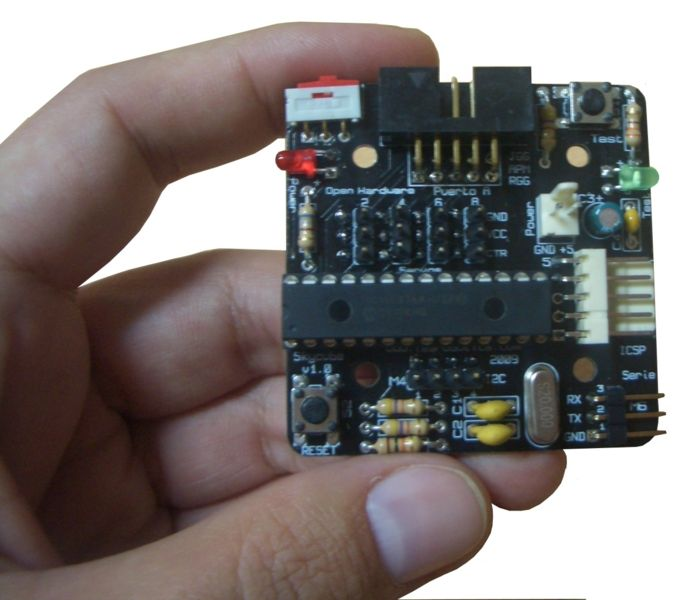
\includegraphics[width=\textwidth]{images/Hardware_skycube.jpg}
                \caption{Skycube board}~\\
                \label{fig:hardware_skycube}
        \end{subfigure}
        ~
        \begin{subfigure}[b]{0.46\textwidth}
                \centering
                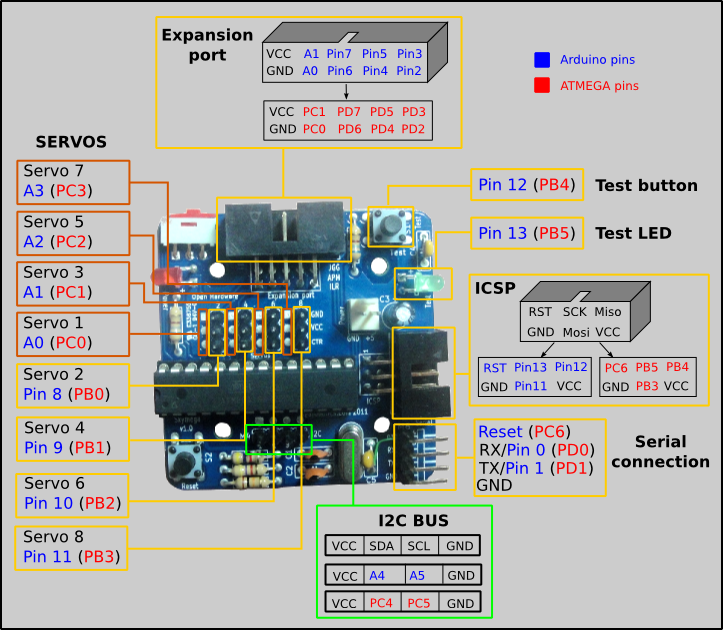
\includegraphics[width=\textwidth]{images/Hardware_skymega_pins.png}
                \caption{Skymega board with a description of the available pins and their functions.}
                \label{fig:hardware_skymega}
        \end{subfigure}
        \caption{Skycube and SkyMega control boards.} 
        \label{fig:hardware_previouswork_boards}
\end{figure}


%%%%%%%%%%%%%%%%%%% SkyMega SMD %%%%%%%%%%%%%%%%%%%%%%%%%%%%%%%%%%%%%%%%%%%%
\subsection{SkyMega SMD}
\label{hardware_electronics_skymegaSMD}

Based on the SkyMega board, a new board was designed and manufactured for this project. This new board improves the original SkyMega design, and solves several problems found on the original design.\\

The main improvements added to the new design are:
\begin{itemize}
	\item The board is populated with surface-mount compoments (SMD) instead of through-hole components (THD). Using SMD components reduces the amount of PCB surface required by each component. This has allowed us to design a cleaner component layout, add extra components and route the board on the top layer, leaving the bottom layer entirely as a ground plane, reducing electrical noise and interferences.
	
	\item A linear, Low-Dropout (LDO) regulator was added to the circuit in order to have a stable 5V supply to the microcontroller. A stable supply is required, for example, if using the analog inputs to measure a voltage. In this case, if the supply is not constant, the measured values will not have a common reference and will vary even if the voltage measured is the same.
	
	\item The supply for the hobby servos has been split into two different power connectors. One of them supplies the LDO regulator that powers the microcontroller and 4 of the 8 servos that the board allows to use, whereas the other connector supplies the remaining 4 servos. The reason the supply has been split is because the hobby servos consume a high amount of current, and the inductive component generated by the DC motor introduces a large amount of noise in the power lines, that even resets the microcontroller when the 8 servos are connected to a single supply in the original SkyMega board. To reduce the effect of the motors on the power supply of the microcontroller,  a capacitor was added next to each servo connector, and the power for the servos is supplied directly from the connector, not passing through the LDO regulator, so the regulated line is as clean as possible.
	
	\item The expansion port has been split into several smaller headers, to reduce the space occupied by the connector. A extra header has been added on the botton of the board for the connection with a optional bluetooth serial transceiver.
	
	\item Two LEDs for power indication on both supplies and two LEDs for serial port transmission signalling were added.
\end{itemize}

The boards were designed with KiCad and sent to be manufactured in SeeedStudio, a chinese manufacturer for very small batches of PCB prototypes. When they arrived, they were assembled by hand, and tested. The resulting assembled boards can be seen in figure \ref{fig:hardware_skymegasmd}.


\begin{figure}[h]
		\centering
        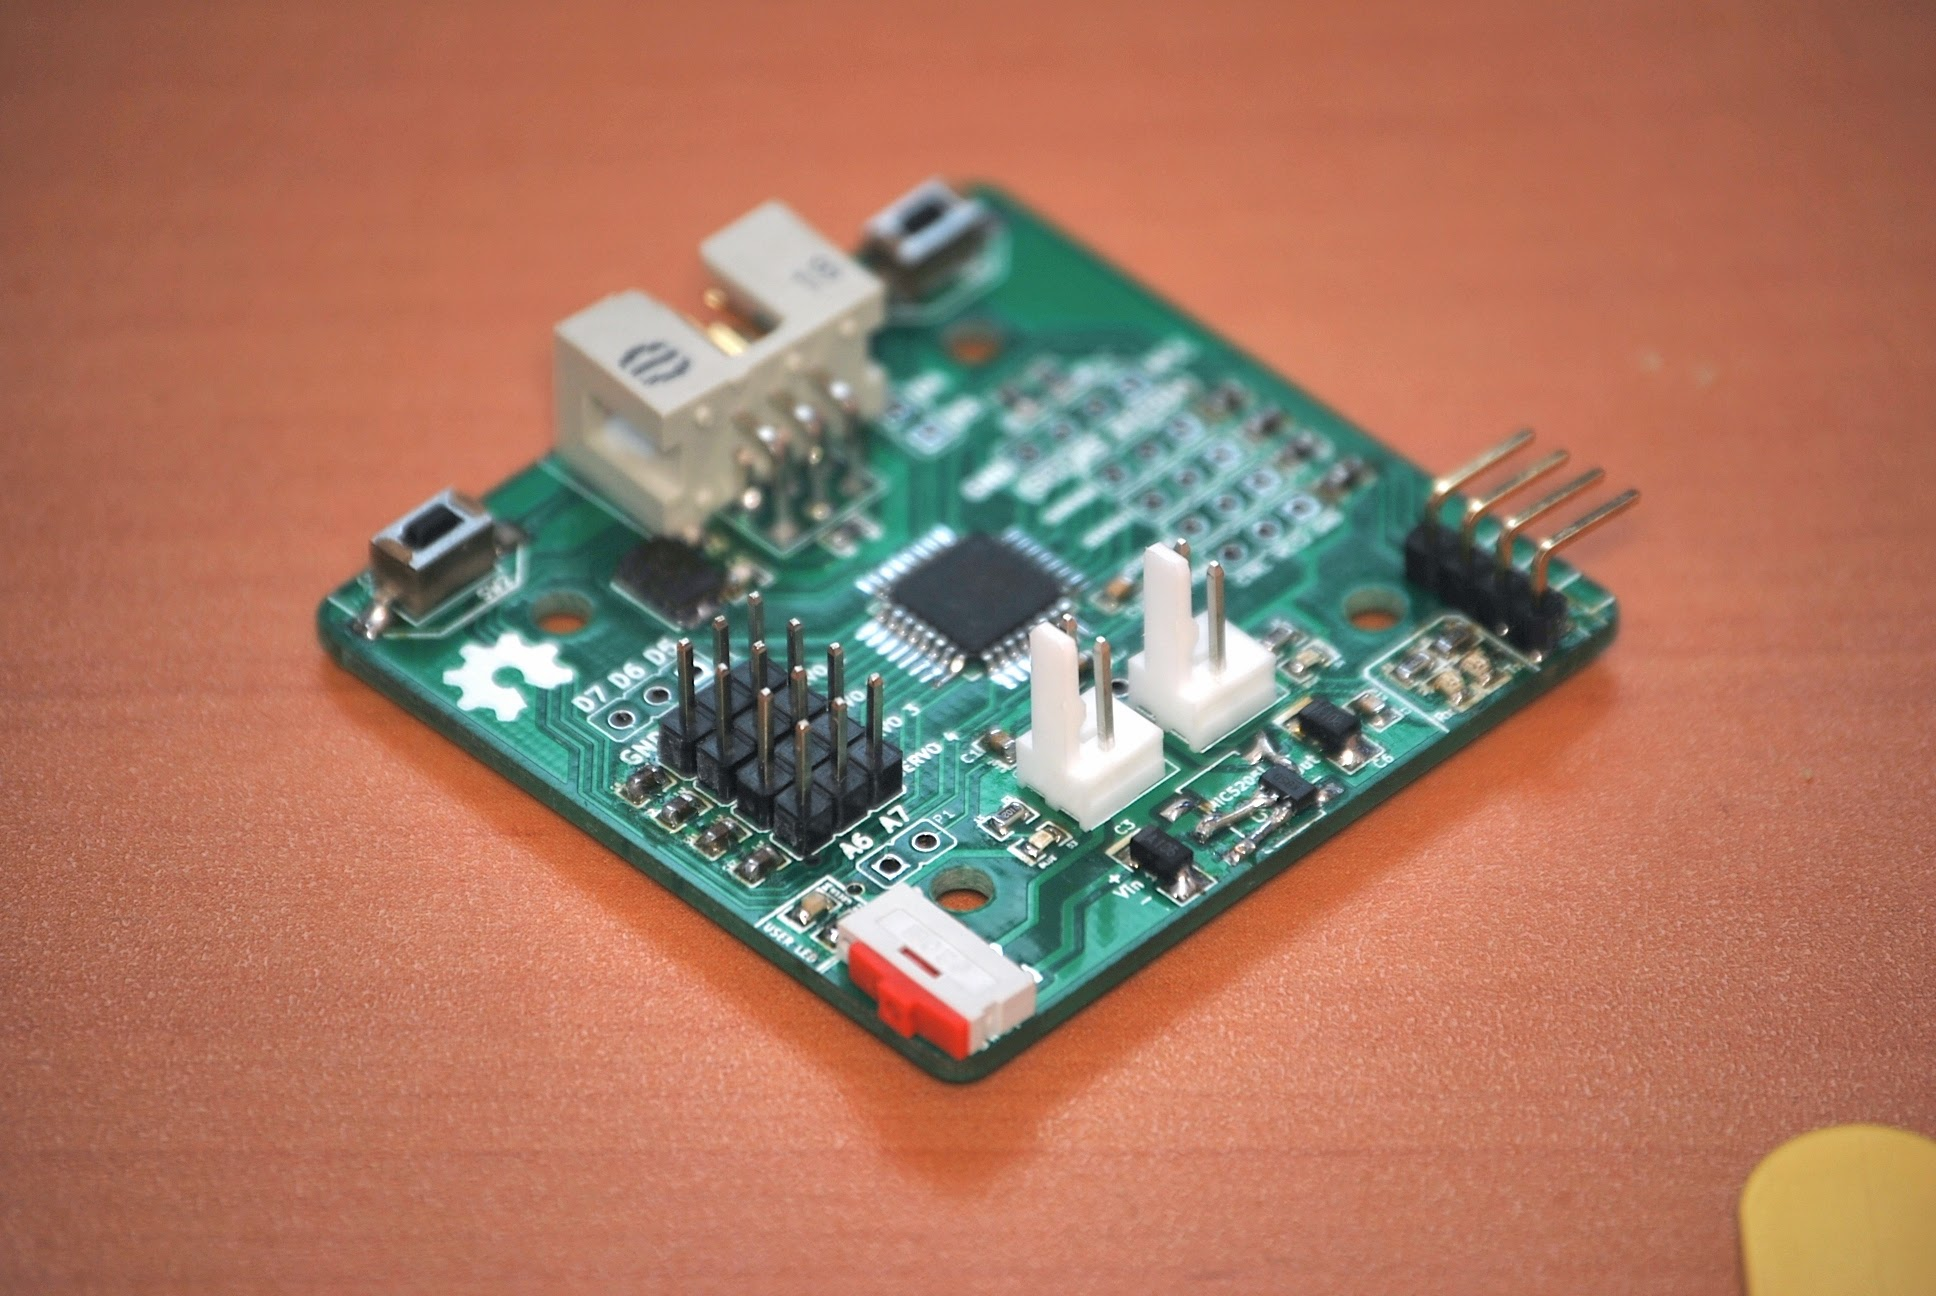
\includegraphics[width=0.55\textwidth]{images/Hardware_skymegasmd.jpg}
        \caption{Assembled SkyMegaSMD}
        \label{fig:hardware_skymegasmd}
\end{figure} 


\section{Other module components}
\label{hardware_electronics_other}

Apart from the control board, the modular robot requires other elements for actuation, communication and power. In this section, we will discuss those elements.

\subsection{Hobby Servomotor}
A servomotor is a motor whose position, velocity or acceleration can be precisely controlled. A servo motor includes, in addition to the motor, a sensor por position feedback and a controller that uses that feedback for controlling the output.\\

For this robot, we have chosen Futaba 3003s hobby servos, that are cheap servomotors intended for Radio Control vehicles. These servos were selected because of their lower price compared with more advanced servos intended for robotics and their availability.\\

These servos are composed by a small DC motor coupled to a plastic reduction gearbox. The output shaft is connected to a potentiometer for position feedback, and the motor is controlled by a controller board placed inside the servo, that takes as input signal a pulse-width modulated signal (PWM). These signal controls the position of the servo output, that restricted from 0º to 180º, as a function of the width of a periodic pulse of 50Hz. With a pulse of 0.3ms of width, the servo joint is placed at one of its extremes, and with a pulse of 2.3ms the servo axis moves to the other extreme. Intermediate values place the shaft in a position between the two extremes. For example, to place the joint centered at the middle of the range, a pulse of 1.3ms has to be sent. If no signal is received, the servo is in standby, and the servo does not oppose to external movements of the shaft. 

\begin{figure}[h]
		\centering
        \begin{subfigure}[b]{0.54\textwidth}
                \centering
                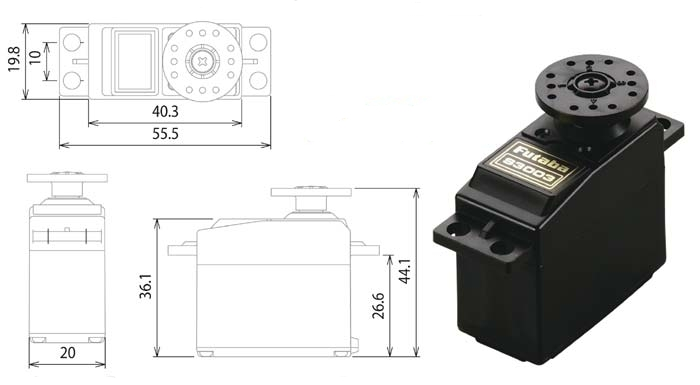
\includegraphics[width=\textwidth]{images/Hardware_futaba3003s_dimensions.jpg}
                \caption{Servo Futaba3003s and dimensions}
                \label{fig:hardware_futaba3003s_dimensions}
        \end{subfigure}
        ~
        \begin{subfigure}[b]{0.43\textwidth}
                \centering
                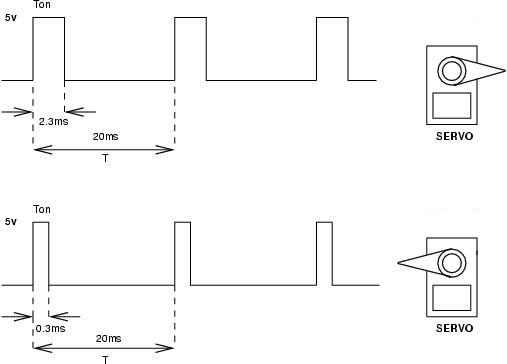
\includegraphics[width=\textwidth]{images/Hardware_futaba3003s_pwm.jpg}
                \caption{PWM signal for position control}
                \label{fig:hardware_futaba3003s_pwm}
        \end{subfigure}
        \caption{Servo Futaba 3003s} 
        \label{fig:hardware_futaba3003s}
\end{figure}


\subsection{USB-to-Serial converter cable}

For firmware upload and communication with the control board, a serial connection with the computer is used. As nowadays most computers do not have a serial connector, a converter is required to connect the serial port of the control board to a USB port on the computer. This converter translates both protocols and allows communication between the computer and the board. As the computer does not have an actual serial port, this port is simulated in software on the computer.\\

The adapter used in the robot is a cable that integrates a FTDI FT232RL USB/serial chip, which translates the USB communications sent by the computer to the TTL RS-232 signals (RX, TX, CTS, RTS) used by the Universal Asynchronous Receiver/Trasmitter (UART) of the microcontroller. The UART is the peripheral of the microcontroller used for serial communication with multiple communication standards, data formats and transmission speeds.\\

\begin{figure}[h]
		\centering
        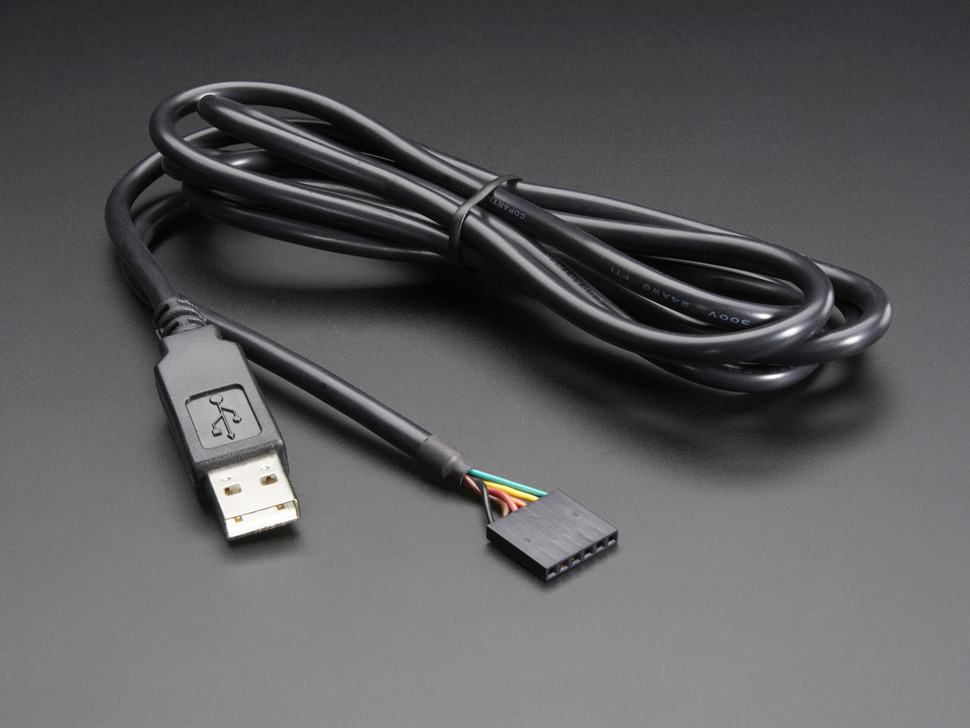
\includegraphics[width=0.5\textwidth]{images/Hardware_ftdi.jpg}
        \caption{USB-to-Serial converter cable}
        \label{fig:hardware_ftdi}
\end{figure} 


\subsection{LiPo Battery}

In order to be autonomous, the robot has to carry its own batteries for power. The batteries used for this robot are Lithium Polymer (LiPo) batteries. These batteries are rechargeable, and offer a very good ratio capacity / weight.\\

 Each cell of a LiPo battery outputs around 4.2V when charged, and they are combined in parallel for a higher capacity or in series for a higher voltage. The number of cells is series is indicated in the battery with a number followed by the letter `S'. A 1S battery has one cell, and will output 4.2V when charged, whereas a 2S has two cells and will output 8.4V when charged. To extend the lifetime and be able to be charged safely, these cells must be balanced (i.e. they must have a similar internal resistance).\\
 
The capacity of the LiPo battery is measured in mAh, the amount of milliamps that they can supply in an hour at a certain voltage (usually the battery voltage). For example, a 1200 mAh battery can supply 1.2A during one hour, or 0.6A during two hours, etc. The maximum discharge rate allowed by the battery is expressed as a number followed by the letter `C', that multiplied by the capacity gives the maximum current that can be drawn. A 10C, 1200mAh battery can supply up to $10 \cdot 1.2 = 12A$.\\

The advantages of LiPo batteries are their high capacity / weight ratio, as mentioned before, and the high discarge current that they can support, and the main drawbacks are that they have to be charged with a specialized charger, as all the cells must be kept balanced to prevent them to ignite.\\

For this project, a 3S (12.6V) battery was used, with a capacity of 2200mAh and a maximum discharge rate of 20C ($20 \cdot 2.2 = 44A$).

\begin{figure}[h]
		\centering
        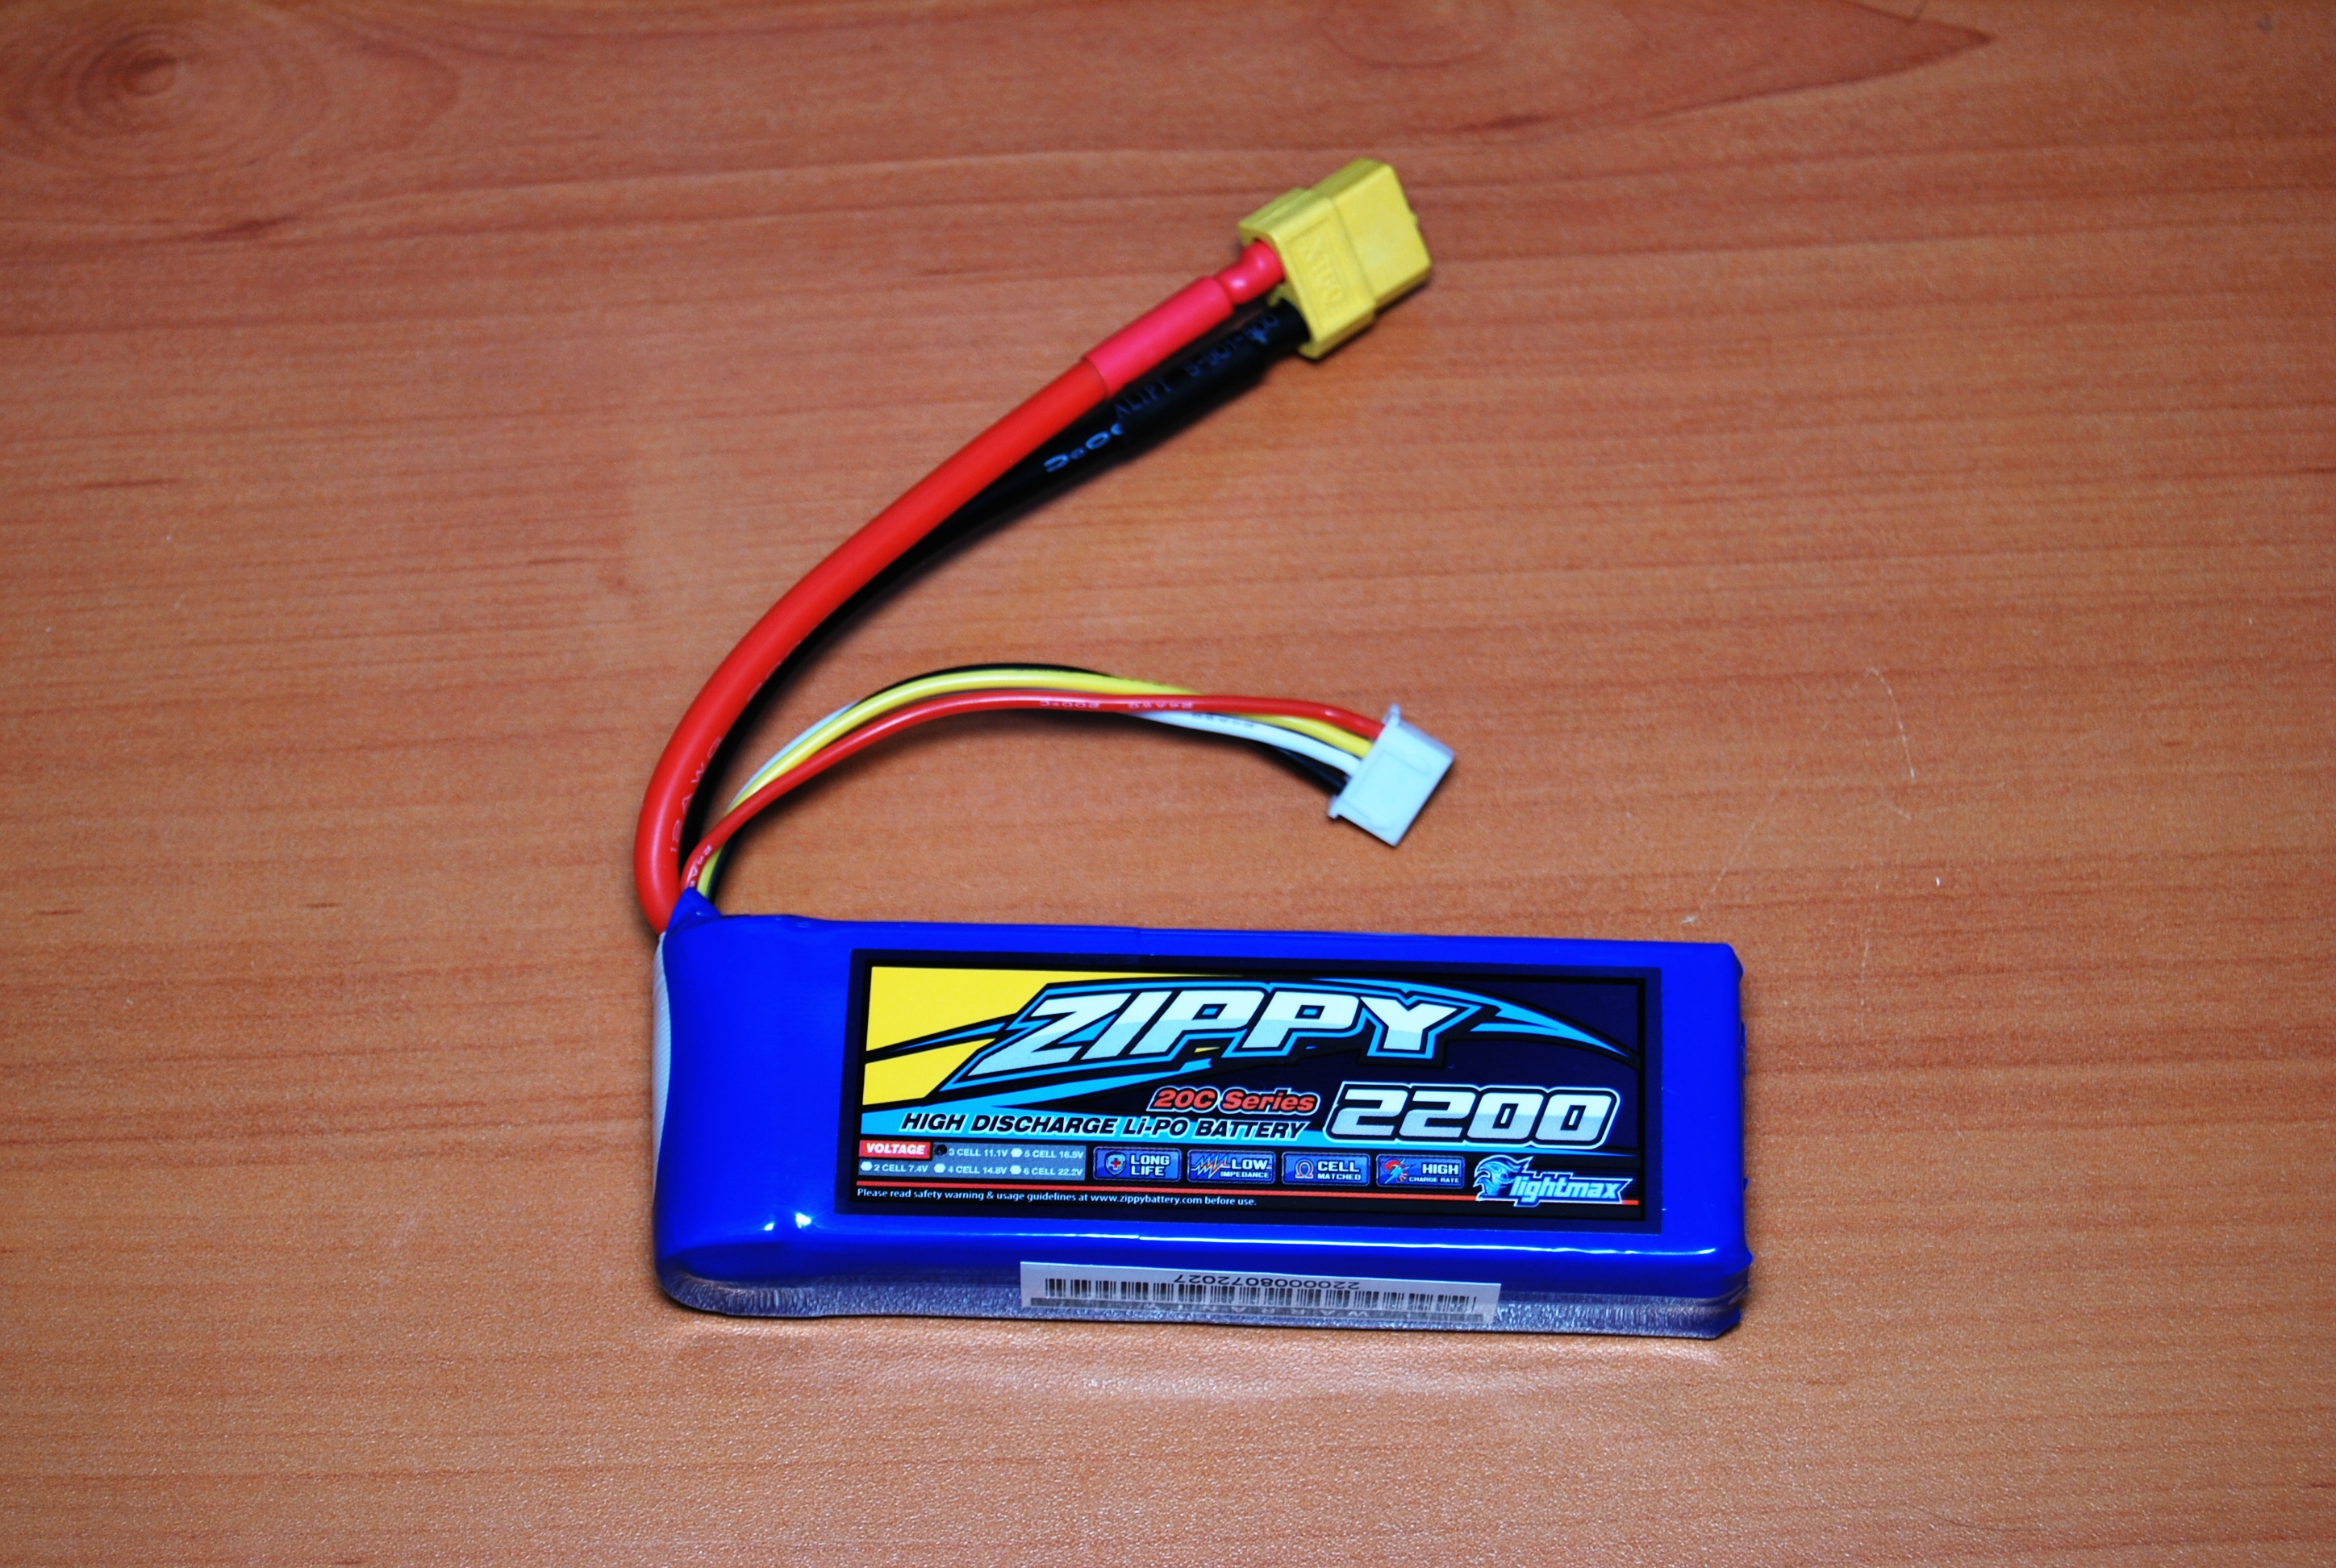
\includegraphics[width=0.55\textwidth]{images/Hardware_lipo.jpg}\\
        \caption{LiPo battery 3S 2200mAh}
        \label{fig:hardware_lipo}
\end{figure}

\subsection{UBEC}

The 3S LiPo battery supplies 11.1V, but the servos and the control board both work at 6V. In order to adapt the supply voltage to the suitable levels, a UBEC is used. A UBEC is a switch-mode DC to DC converter very common in RC planes and helicopters to supply power to the control board, transmitter and servos that actuate the control surfaces from the same battery that powers the motors, eliminating the necessity of having a dedicated battery with a lower voltage for them.\\

The UBEC chosen for this robot is a Turnigy UBEC that can supply up to 8A (or up to 15A for a very short period of time). It accepts input voltages from 6V to 12.6V, which correspond to 2S or 3S batteries, and has a selectable output of 5V or 6V. It also has LEDs for indication of the current battery level.\\

\begin{figure}[h]
		\centering
        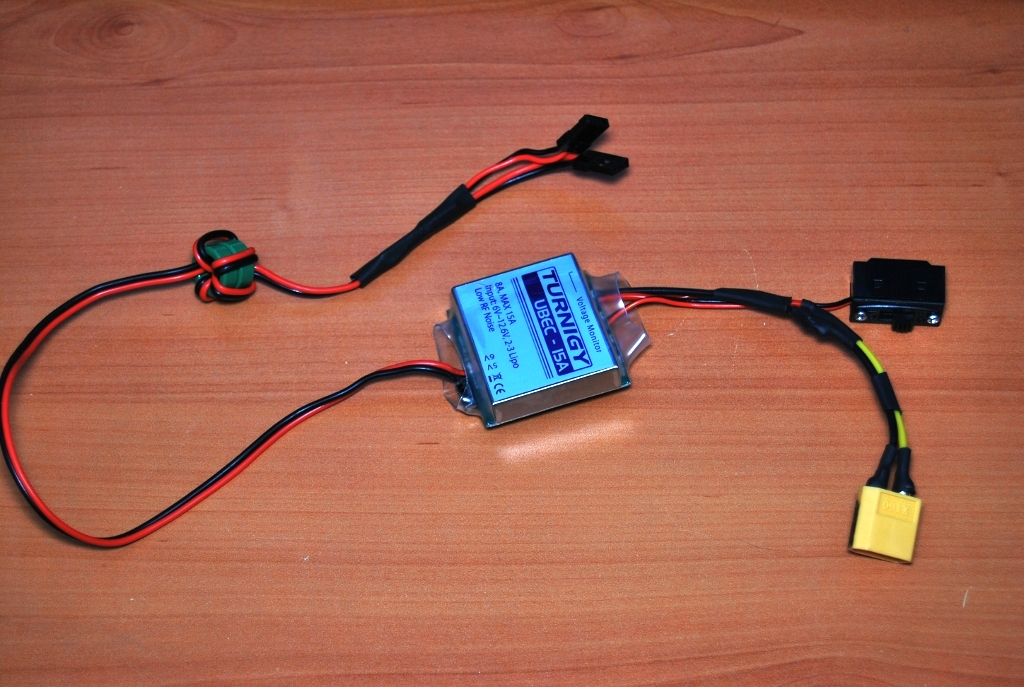
\includegraphics[width=0.55\textwidth]{images/Hardware_ubec.jpg}\\
        \caption{UBEC Turnigy 8A}
        \label{fig:hardware_ubec}
\end{figure} 


\subsection{Bluetooth module}

The cables connected to the robot for power and communication limit the movement of the robot, affecting to the resulting gait. The cables for power can be removed by adding batteries to the robot and, for removing the cable used for communication, a Bluetooth module was tested.\\

Bluetooth is a wireless technology standard used for data transmission over short distances, using the 2.4 GHz to 2.485 GHz band. It is used for communication between fixed and mobile devices, and between mobile devices, for building wireless personal area networks (WPANs). It was invented by Ericsson, as a wireless alternative of wired RS-232 communications.\\

The Bluetooth module used was a JY-MCU, which includes a HC-06 bluetooth transceiver. These modules are very cheap, and they are able to transmit a serial connection over bluetooth using the RFCOMM protocol, taking care of the bluetooth protocol and implementing a virtual serial data stream. On the other side, the communication range spans only a few meters, but that range is enough for our application.\\

\begin{figure}[h]
		\centering
        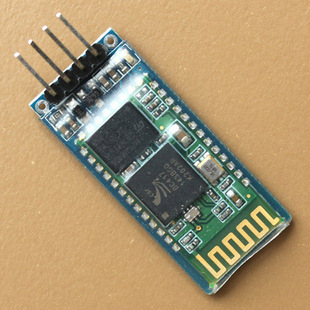
\includegraphics[width=0.3\textwidth]{images/Hardware_jy-mcu.jpg}\\
        \caption{Bluetooth module JY-MCU}
        \label{fig:hardware_bluetooth}
\end{figure} 



%%%%%%%%%%%%%%%%%%% Firmware %%%%%%%%%%%%%%%%%%%%%%%%%%%%%%%%%%%%%%%%%%%%
\section{Firmware}
\label{hardware_firmware}

To control the modular robot from the computer, a very simple firmware was developed. This firmware opens a serial port to connect with the computer and waits for commands. With these commands, the position of the joints can be specified, as well as the state of the onboard LED.\\

Since the number of servos that a single board can drive is limited to 8, for the configurations with more than 8 servos two boards have to be used. These boards are connected to each other using the I2C bus, with a board acting as a master and the other acting as a slave. The master board is also connected to the computer via serial port to receive the commands. The commands are sent from the computer at a certain rate, updating the joint position according to the oscillator output values. Those oscillations generate the locomotion of the modular robot.\\

The steps followed by the firmware are the following:
\begin{enumerate}
	\item The microcontroller UART is configured and the serial port is open. When the robot is ready, it sends a string ``Ok!'' to the computer, indicating that it is waiting for commands. This string is used by the software on the computer to check that the robot is listening to the commands.
	
	\item The microcontroller waits for a command. The received bytes are stored in a buffer and when a command byte is received, the remaining bytes of the command are processed. The start byte is composed of a pattern of 4 bits (0101) followed by 4 bits indicating the command, so all the available bytes for being used as a command go from 0x50 to 0x5F.
	
	\item The command is processed. Currently there are 4 commands available:
		\begin{itemize}
			\item \textbf{0x50}: Set the position of all the joints. After this byte, the firmware expects as many bytes as joints have the robot, each byte containing the angular position of that joint, from 0º to 180º. For a robot with two joints, to be set at 45º and 30º respectively, the command would be: 0x50 0x2D 0x1E.
			
			\item \textbf{0x51}: Set the position on a single joint. This command needs two bytes to be received after the command, the index of the joint to be set and its value. If the third joint of the robot is to be set at 50º, the command would be: 0x51 0x02 0x32 (the joint indexes start with 0, so the third joint has index 2).
		
			\item \textbf{0x52}: Send message to another board. Since the number of servos that a control board can drive is limited to 8, for configurations with more servos two boards have to be connected using the I2C bus. When two boards are connected, the master board can relay messages to the slave board using this command. This command requires the size of the message to be sent to be specified after the command. For example, if the would like to set the third joint of the slave board to 50º (command 0x51 0x02 0x32), we would have to send the following command to the master board: 0x52 0x03 0x51 0x02 0x32.
			
			\item \textbf{0x5F}: Test command. It just toggles the USER LED on the control board, and can be used to test the connection with the board visually.
		\end{itemize}
		
	\item Waits for another command to execute.
\end{enumerate}

The firmware of the slave board has to slightly different, as the commands are received by the I2C bus, instead of the serial port, and it does not accept the ``Send message'' command (0x52), since there is no other board connected to the slave board except for the master board. This slave board firmware has not been developed to to time limitations, and is left as future work.\\

The use of this firmware implies that the modular robot is a dummy robot: the actual controller that generates the joint positions is run on the computer, and the robot control board only sets those values to the actual robot in order to check the resulting locomotion.\\
